\documentclass[pdflatex,11pt]{aghdpl}
% \documentclass{aghdpl}               % przy kompilacji programem latex
% \documentclass[pdflatex,en]{aghdpl}  % praca w języku angielskim
\usepackage[polish]{babel}
\usepackage[utf8]{inputenc}
\usepackage{float}

% dodatkowe pakiety
\usepackage{enumerate}
\usepackage{listings}
\lstloadlanguages{TeX}

\lstset{
  literate={ą}{{\k{a}}}1
           {ć}{{\'c}}1
           {ę}{{\k{e}}}1
           {ó}{{\'o}}1
           {ń}{{\'n}}1
           {ł}{{\l{}}}1
           {ś}{{\'s}}1
           {ź}{{\'z}}1
           {ż}{{\.z}}1
           {Ą}{{\k{A}}}1
           {Ć}{{\'C}}1
           {Ę}{{\k{E}}}1
           {Ó}{{\'O}}1
           {Ń}{{\'N}}1
           {Ł}{{\L{}}}1
           {Ś}{{\'S}}1
           {Ź}{{\'Z}}1
           {Ż}{{\.Z}}1
}

%---------------------------------------------------------------------------

\author{Tomasz Górny}
\shortauthor{T. Górny}

\titlePL{Opracowanie systemu inwestycyjnego opartego na wybranych japońskich technikach analizy wykresów}
\titleEN{Development of the investment system based on selected investment analysis techniques of Japanese charts}

\shorttitlePL{Opracowanie systemu inwestycyjnego opartego na świecach japońskich} % skrócona wersja tytułu jeśli jest bardzo długi
\shorttitleEN{Development of the investment system based on the Japanese candles}

\thesistypePL{Praca magisterska}
\thesistypeEN{Master of Science Thesis}

\supervisorPL{dr inż. Mirosław Gajer}
\supervisorEN{Mirosław Gajer Ph.D}

\date{2012}

\departmentPL{Katedra Automatyki}
\departmentEN{Department of Automatics}

\facultyPL{Wydział Elektrotechniki, Automatyki, Informatyki i Elektroniki}
\facultyEN{Faculty of Electrical Engineering, Automatics, Computer Science and Electronics}

\acknowledgements{}



\setlength{\cftsecnumwidth}{10mm}

%---------------------------------------------------------------------------

\begin{document}

\titlepages

\tableofcontents
\clearpage

\chapter{Wstęp}
\label{chap:wstep}
\paragraph{}
Trafne prognozowanie zachowania się rynków finansowych to zadanie niezwykle trudne. Stworzono wiele teorii na ten temat, z których każda ma swoich wiernych zwolenników. W ramach istniejących ideii zostały zbudowane metody, których realizacja może w różnym stopniu pozwolić inwestorowi przewidzieć zachowanie na giełdzie, a tym samym zapewnić mu zysk, bądź uchronić przed stratami. Informacje płynące z większości algorytmów wspierających inwestycje muszą być poparte szeroką wiedzą na temat danego rynku. Spowodowane jest to faktem, iż na ceny notowań wpływa wiele czynników, których interpretacja wymaga doświadczenia oraz znajomości tematu. Poza nabytą wiedzą z zakresu zasad funkcjonowania danej giełdy należy posiadać bezwzględną dyscyplinę przy kierowaniu się określonym algorytmem inwestycyjnym. Emocje i stres, towarzyszące ryzyku utraty środków pieniężnych, przeważnie dorowadzają inwestorów do nietrafnych wyborów, pomimo założonej strategii. Nieustanny postęp komputeryzacji daje okazję do konstruowania coraz to lepszych aplikacji do wspierania działań gracza giełdowego. Tego rodzaju systemy coraz częściej są stosowane z powodzeniem na wielu rynkach. Specjalistyczne aplikacje upraszczają pracę analityka, dostarczając wielu narzędzi i algorytmów. W istotnym stopniu redukują one czas potrzebny na analizę danych. Dodatkowo tego typu programy niwelują emocje, zapewniają dyscyplinę podczas podejmowaniu decyzji oraz są konsekwentne w ramach wybranej strategii. Dzięki temu inwestor może zwiększać swoje zyski przy jednoczesnym minimalizowaniu ewentualnych strat. Wyniki analiz, oferowane przez systemy inwestycyjne, są generowane za pomocą szeregu algorytmów. Procedury te zaiplementowane są na podstawie teoretycznych teorii inwestowania. Wraz z powstawaniem nowych teorii oraz strategii, programiści starają się stworzyć algorytmy, które będa je realizowały.  
\section{Cele pracy}
\paragraph{}
Celem pracy jest stworzenie automatycznej strategii inwestycyjnej, prognozującej kursy walut na rynku Forex za pomocą algorytmów opartych na wybranych japońskich technikach analizy wykresów. Główne wymagania:
\begin{itemize}
\item
zaimplementowanie algorytmów rozpoznających główne formacje świec japońskich
\item
optymalizacja algorytmów pod kątem maksymalizacji zysku
\item
zbudowanie strategii realizającej automatyczne transakcje bazujące na rozpoznanych wzorcach świec japońskich
\item
ocena sprawdzalności sygnałów płynących z japońskich technik analizy wykresów
\end{itemize}
\section{Zawartość pracy}
\paragraph{}
W rozdziale drugim zostaną przedstawione teoretyczne podstawy niezbędne do projektowania aplikacji. Opisane zostaną założenia, zasady oraz podstawy funkcjonowania analizy technicznej. Omówione zostaną rodzaje metod analizy technicznej stosowane przez inwestorów. Przedstawione zostaną możliwości istniejących na rynku systemów transakcyjnych.

Trzeci rozdział dotyczy sposobu, w jaki zostanie zrealizowany projekt systemu, prognozującego ceny akcji. Przedstawione zostaną wymagania stawiane tego rodzaju aplikacji oraz główne założenia przy budowaniu niniejszego programu. W rozdziale zawarte zostaną diagramy UML. Omówione zostaną kwestie dotyczące procedury działania aplikacji.

Rozdział czwarty zawiera informacje na temat implementacji projektu. Przedstawia narzędzia użyte do stworzenia aplikacji. Zaprezentowana zostanie budowa bazy danych oraz interfejsu użytkownika. Rozdział omawia główne funkcje programu pod kątem sposobu ich działania.

W rozdziale piątym zostaną przedstawione wyniki działania algorytmów oraz ocena ich skuteczności w przewidywaniu przyszłych wartości notowań na Warszawskiej Giełdzie Papierów Wartościowych.  

Rozdział szósty jest podsumowaniem pracy. Omawia aspekty postawionego problemu, które zostały spełnione, jak również te, których nie udało się rozwiązać. W rozdziale wyszczególnione zostały wymagania projektu, które udało się zrealizować. Dodatkowo rozdział zawiera wnioski na temat projektu oraz jego szczególne walory.
\chapter{Podstawy teoretyczne}
\label{chap:teoria}

\section{Rynek Forex}
\label{sec:forex}
\paragraph{}
Handel pieniędzmi rozpoczął się już we wrzesnym średniowieczu. Tamtejsi kupcy i bankierzy jako pierwsi używali kwitów wymiany umożliwiających rozwój i uelastycznienie handlu międzynarodowego. Współczesny rynek wymiany walutowej przechodzący przez okresy dużej zmienności i relatywnej stabilności uformował się dopiero w XX wieku. Londyn w latach trzydziestych XX wieku stał się głównym centrum wymiany walut. Jednocześnie funt brytyjsk rósł w siłę, należąc do najsilniejszych. Druga wojna światowa doprowadziła brytyjską ekonomie do skraju bankructwa. W tym samym czasie wzrostała pozycja Stanów Zjednoczonych. Kraj niezniszczony wojną zyskał silną pozycję ekonomiczną. W 1944 roku na mocy porozumienia z Bretton Woods między Stanami Zjednoczonymi, Wielką Brytanią oraz Francją, dolar amerykański stał się bazową walutą kapitalistycznych krajów. Wszystkie waluty oraz złoto zostały powiązane z walutą bazową. W ten sposób dolar stał się główną walutą całego finansowego świata. W ramach porozumienia powstał Międzynarodowy Fundusz Monetarny, który przyczynił się do finansowania byłych socjalistycznych krajów.\cite{9} 

W latach siedemdziesiątych kursy walut zostały uwolnione od cen złota. Wydarzenie to jest momentem powstania rynku wymiany walut jaki znamy do dziś. Termin Forex (ang. Foreign Exchange - wymiana walut) stał się potoczną nazwą największego międzynarodowego rynku na świecie na którym odbywa się wymiana walut. Wielkość dziennych obrotów przekracza 1,9 biliona USD, co stanowi trzykrotność łącznych obrotów na amerykańskim rynku akcji i obligacji. Forex jest rynkiem OTC (Over The Counter), co oznacza, że nie ma jednego miejsca usytuowania na świecie gdzie dokonuje się wszystkich operacji na tym rynku. Handel parami walut odbywa się głównie za pośrednictwem internetu, telefonów, globalnej sieci banków, brokerów, przesiębiorstw oraz inwestorów indywidualnych. Brak określonego miejsca fizycznej lokalizacji rynku walutowego umożliwia mu funkcjonowanie 24 godziny na dobę przez 5 dni w tygodniu, od godziny 23 w niedzielę do godziny 22 w piątek czasu środkowoeuropejskiego. Rynek ten obejmuje swym zasięgiem większość krajów świata, a do największych centrów transakcji walutowych należą Londyn, Nowy Jork i Tokio. Do najwazniejszych walut wymienianych na rynku Forex należą:
\begin{itemize}
\item USD - dolar amerykański
\item EUR - euro
\item GBP - funt brytyjski
\item JPY - jen japoński
\item CHF - frank szwajcarski
\item AUD - dolar australijski
\item NZD - dolar nowozelandzki
\end{itemize}

Olbrzymia liczba uczestników i ich różnorodność sprawia, że rynek walutowy jest najbardziej płynnym rynkiem finansowym świata, a manipulowanie nim jest wręcz niemożliwe, nawet dla takich instytucji jak banki centralne największych państw naszego globu. Sytuacja ta powoduje, że właściwie jedyną determinantą poziomu kursów walutowych jest zachowanie większości uczestników rynku, a nie tylko największych graczy, co sprawia, że inwestor, który trafnie potrafi przewidzieć zachowanie ,,tłumu'' może odnosić na tym rynku ponadprzeciętne zyski.
Jeszcze do niedawna handel na Rynku Forex zarezerwowany był dla ,,rekinów'' świata finansów takich jak banki, fundusze inwestycyjne, duże przedsiębiorstwa, jednakże wraz z rozwojem internetu, możliwość aktywnego uczestniczenia na tym rynku została udostępniona znacznie szerszemu gronu osób. W chwili obecnej praktycznie każdy kto ma komputer z dostępem do internetu może w łatwy sposób rozpocząć swoją przygodę na tym rynku.

Rynk Forex posiada różne odmiany, które charakteryzują się różnym sposobem wymiany walut. Do najważniejszych należa:
\begin{itemize}
\item rynek kontraktów natychmiastowych
\item rynek terminowy
\item rynek opcji
\end{itemize}

Na najpopularniejszym rynku kontraktów natychamiastowych zlecenia na dostawy, określonych ilości walut, są wykonywane bezzwłocznie, a późniejsze zmiany kursu wpływają na wartość kontraktu w czasie rzeczywistym. Na rynku terminowym waluty dostarczane są w określonym momencie w przyszłości po cenie ustalanej obecnie. Z tego rynku korzystają eksporterzy i importerzy obliczając rzeczywiste koszty eksportowanych i importowanych w przyszłości towarów względem zmian kursów walut. Rynek opcji to rynek, w którym handlowi podlegają prawa do wykupu lub sprzedaży w określonym czasie i po określonej cenie instrumentów finansowych. 

Giełda Forex posiada wiele zalet i oferuje niesamowite korzyści w stosunku do innych rynków. Poniżej zostały przedstawione najważniejsze atuty, które zachęcają do inwestowania na omawianym rynku:
\begin{itemize}
\item Łatwy dostep. 
Do niedawna nawet osoby z pokaźnym kapitałem nie mogły w praktyce inwestować swoich pieniędzy na rynku Forex. Obecnie wraz z rozwojem technologii internetowych, powstały możliwości elektronicznego łączenia małych i rozbijania dużych zleceń. Dzięki temu można zacząć inwestowanie na tym rynku nawet z niewielkimi pieniędzmi.
\item Wyjątkowa płynność. 
Forex jest ogromnym rynkiem, co sprawia, że jest również rynkiem wyjątkowo płynnym. Oznacza to, że można złożyć zlecenie mając pewność, że zostanie natychmiast zrealizowane. Dzięki tak wielkiej płynności rynek ten jest odporny na wszelkie manipulowanie kursami.
\item Handel przez 24 godziny na dobę. 
W odróżnieniu od innych rynków czy giełd papierów wartościowych, Forex jest czynny od poniedziałku do piątku przez 24 godziny na dobę. 
\item Zarabianie zarówno przy trendzie zwyżkowym jak i zniżkowym.
Na rynku akcji mamy możliwość zarabiania przede wszystkim na trendzie wzrostowym. Jedną z największych zalet Forexu jest możliwość osiągania zysków zarówno przy wzroście jak i przy spadku danej waluty.
\item Możliwość ,,lewarowania'' pozycji.
Duża dźwignia handlowa, dochodząca do 200 : 1, oznacza że depozytem w wysokości np. 100\$ można kontrolować kupno lub sprzedaż walut o wartości 20.000\$. Jeśli przy takim lewarze kurs zakupionej waluty wzrośnie tylko o 0,1\%, zysk wyniesie 20\$, czyli 20\% w stosunku do kwoty przez nas zainwestowaną. Niestety niewielkie zmiany w przeciwną stronę mogą powodować szybkie wyzerowanie się rachunku.
\end{itemize}

Inwestując na rynku Forex można spotkać się z wieloma specjalistycznymi terminami. Poniżej zostanie objaśnione znaczenie najważniejszych pojęć.
\begin{itemize}
\item Lot to jednostka określająca minimalna ilość danej waluty, którą można wykupić na danej platformie i danym typie konta. W większości przypadków dla kont mini wartość ta wynosi 10.000, a dla kont standardowych 100.000. Przy dźwigni 200:1 za jeden lot stanowiący 10.000 jednostek waluty, do otwarcia transakcji wymagane jest 50\$. Na koncie standardowym z lewarem 100:1 oraze lotem wynoszącym 100.000, wymagane jest 1000\$.
\item Spread to termin pochodzący z angielskiego i oznacza różnicę między cenami kupna i sprzedaży danej pary walutowej. Jest to prowizja transakcji, którą pobiera broker. Każda para walutowa ma określony swój własny spread, który w zależności od brokera i konta może być zmienny w czasie lub stały.
\item Luka cenowa to różnica pomiędzy ceną zamknięcia świecy poprzedniej, a ceną otwarcia kolejnej świecy. Spowodowana jest nagłymi zmianami kursów. Szczególnie niebezpieczna dla inwestora, może okazać się luka cenowa tworząca się w trakcie trwania weekendu. Istotny jest fakt, że zlecenia stop loss nie są realizowane w trakcie weekendu. Dlatego jeśli pojawiająca się luka jest w kierunku przeciwnym do pozycji inwestora, może spowodować ona wyzerowanie się konta, a nawet zaciągnięcie kredytu. Warto zauważyć, że pozytywna luka cenowa, której kierunek zgadza się z kierunkiem pozycji inwestora zapewni maksymalnie zysk ustawiony limitem take profit.  
\item Dźwignia to narzędzie, dzięki któremu małą sumą pieniędzy można kontrolować pozycję o znacznie większej wartości. Jest to relacja pomiędzy kapitałem o stałym oprocentowaniu pożyczonym przez firmę brokerską (kredyt), a wartością zainwestowanego kapitału (depozyt).
\item Pozycja krótka. Jest to transakcja sprzedaży danej ilości waluty po okreśłonej cenie. Zajmując pozycję krótką oczekuje się spadku cen. 
\item Pozucja długa. To transakcja zakupu danej ilości waluty po określonej cenie. W tym wypadku zysk jest osiągany przy zwyżkach cen.
\end{itemize}

\section{Analiza techniczna}
\label{sec:analizatechniczna}
\paragraph{}
Analiza techniczna to badanie zachowań rynku, przede wszystkim przy użyciu wykresów. Celem badania jest przewidywanie przyszłych trendów cenowych\cite{5}. Metody analizy technicznej na podstawie oceny historycznego kształtowania się cen starają się przewidzieć przyszłe wraz ze zmianami w kierunkach trendów. Narzędziem analizy technicznej, prezentującym wszystkie czynniki wpływające na ceny akcji, jest akcjogram. Akcjogram to wykres przedstawiający kształtowanie się ceny akcji w określonym odcinku czasowym. Na podstawie analizy wykresów prezentujących zmiany cen na giełdzie można odnaleźć cykliczne konfiguracje, pozwalające na budowanie prognoz przyszłych trendów cen akcji. 

Pierwsze z podstawowych założeń analizy technicznej mówi, że rynek dyskontuje wszytko. Zwolennicy analizy technicznej uważają, że wszystkie czynniki wpływające na cenę akcji znajdują odzwierciedlenie w jej cenie\cite{5}. Wynika z tego, że badanie kształtowania się cen jest rozwiązaniem całkowicie wystarczającym do prognozowania. Dlatego też w analizie technicznej dane finansowe odgrywają znikomą rolę. Kolejnym wnioskiem płynącym z tej tezy jest stwierdzenie, że zjawiska giełdowe wyprzedzają w czasie zjawiska ekonomiczne. Informacje płynące z analiz finansowych mogą dawać zbyt opóźnione sygnały. Z tego powodu w rozwiniętych gospodarkach to giełdy papierów wartościowych stanowią wskaźnik rozwoju gospodarczego danego kraju.

Drugim istotnym założeniem w analizie technicznej jest przekonanie o istnieniu trendów cen. Głównym celem badania wykresów cen jest rozpoznanie trendów w ich początkowych fazach. Pozwala to na osiąganie wyższych zysków z przeprowadzonych transakcji. Większość metod w analizie technicznej przeznaczona jest do rozpoznawania trendów oraz podążania za już istniejącymi. Dodatkowo ważnym elementem tego założenia jest stwierdzenie, że trend wykazuje silniejszą tendencję do kontynuowania swojego biegu w dotychczasowym kierunku, aniżeli do jego zmiany\cite{5}. Podejście oparte na analizie trendu bazuje na wykorzystaniu aktualnego trendu, do czasu sygnałów mówiących o jego zmianie.

Ostatnie z kluczowych założeń analizy technicznej dotyczy powtarzającej się historii. Oznacza to, że aby być w stanie prognozować przyszłość, należy zanalizować przeszłość. Metody analizy technicznej znane są od lat. Formacje cenowe, sygnały płynące ze wskaźników i zachowania trendów sprawdziły się w przeszłości, dlatego założono, że potwierdzą sie w przyszłości\cite{5}. 

Dla zrozumienia metod analizy technicznej, które będą przytoczone w dalszej części tego rozdziału, należy pamiętać o podstawowych zasadach przedstawionych przez Pawła Perza:
\begin{itemize}
\item cena akcji jest określana przez relacje między popytem a podażą
\item zmiany w popycie i podaży odzwierciedla akcjogram
\item w zdecydowanej większości przypadków ceny akcji zmieniają się zgodnie z trwającym przez pewien czas trendem
\item zmiany w trendzie wynikają ze zmian w popycie i podaży
\item zmiany mają charakter prawidłowości i podlegają powtarzalności 
\end{itemize}
Wyróżnia sie trzy podstawowe metody analizy technicznej:
\begin{enumerate}
\item analiza trendów cen akcji
\item analiza formacji
\item analiza wskaźników technicznych
\end{enumerate}

W metodzie analizy trendów ocenia się ogólną tendencję rozwojową cen akcji. Gdy trend zostanie rozpoznany, próbuje sie prognozować moment zwrotu trendu\cite{8}. Trend na akcjogramie zostaje wyznaczony poprzez połączenie lokalnych maksimów lub minimów jedną linią prostą. Im więcej takich punktów można połączyć linią trendu, tym większe prawdopodobieństwo prawidłowego wytyczenia trendu i jego większe znaczenie. Przy trendzie rosnącym używamy lokalnych minimów, zaś przy trendzie malejącym lokalnych maksimów. Ważnym elementem analizy trendów są linia oporu i wsparcia. Linia oporu to prosta łącząca maksima na akcjogramie. Prosta ta wyznacza granicę, do której kursy akcji dochodziły, jednak nigdy nie przekraczały jej istotnie. Analogicznie linia wsparcia to prosta linia trendu poprowadzona po minimach, gdzie ceny akcji nie spadały znacząco poniżej jej poziomu. Badając aktualne położenie cen akcji względem trendu, linii oporu i wsparcia oraz kanałów trendowych, które tworzą te linie, można podejmować decyzje o ewentualnym kupnie bądź sprzedaży. Dodatkowo inwestorzy powinni dokonywać transakcji zgodnie z kierunkiem trendu tzn. w trakcie trendu wzrostowego powinni zajmować pozycję długą (kupować dany instrument), w trakcie trendu spadkowego powinni zajmować pozycję krótką (sprzedawać dany instrument). W trendzie horyzontalnym wskazane jest unikanie zawierania transakcji\cite{6}.

Drugim ważnym elementem analizy technicznej jest analiza formacji. Dzięki wieloletnim badaniom kształtowania się cen akcji na giełdach, zauważono powtarzające się zachowania kursów, układających sie na wykresach w charakterystyczne formacje. Poprawne rozpoznanie formacji daje możliwość znalezienia przybliżonego momentu zakupu lub sprzedaży akcji. 

Szczególnym przypadkiem analizy formacji jest rozpoznawanie sekwencji ''świec,,. Metoda ta wywodzi się z Japonii, gdzie jest stosowana od wielu lat, a w ostatnim czasie zdobyła popularność również na Zachodzie. Analiza formacji świecowych może w znacznym stopniu usprawnić posługiwanie się popularnymi wskaźnikami technicznymi oraz uwiarygodnić ich wskazania\cite{3}. Analiza świecowa dotyczy dwóch różnych zagadnień. Po pierwsze zajmuje się odpowiednim prezentowaniem danych na wykresie, a po drugie rozpoznawaniem określonych sekwencji świec, które mają znaczenie prognostyczne. Do konstrukcji wykresów świecowych wymagane są: cena otwarcia, zamknięcia, cena minimalna oraz maksymalna. Często istnieje brak danych o cenach otwarcia, dlatego też w takim przypadku można zastępować je cenami zamknięcia z dnia poprzedniego. Wymienione dane na wykresach świecowych są prezentowane w sposób o wiele bardziej czytelny, niż w przypadku innego typu wykresów. Na rysunku \ref{swieca} przedstawiono przykład wykresu świecowego. Od razu widać, skąd wzięła sie jego nazwa: dane z dnia przypominają świece z knotem. Prostokąt, inaczej zwany korpusem, reprezentuje różnicę pomiędzy ceną otwarcia i cena zamknięcia. W klasycznej teorii istnieją dwa kolory korpusu: biały oznacza, że cena zamknięcia jest wyższa od ceny otwarcia, a korpus czarny mówi o tym, że cena zamknięcia jest mniejsza od ceny otwarcia. Na rysunku \ref{swieca} kolory korpusów zostały odwrócone. Czarny pełni funkcję białego, a biały czarnego korpusu z klasycznej teorii świecowej. Knoty, inaczej zwane cieniami, to linie powyżej i poniżej korpusu. Reprezentują cenę minimalną oraz maksymalną. 
\begin{figure}[ht]
\begin{center}
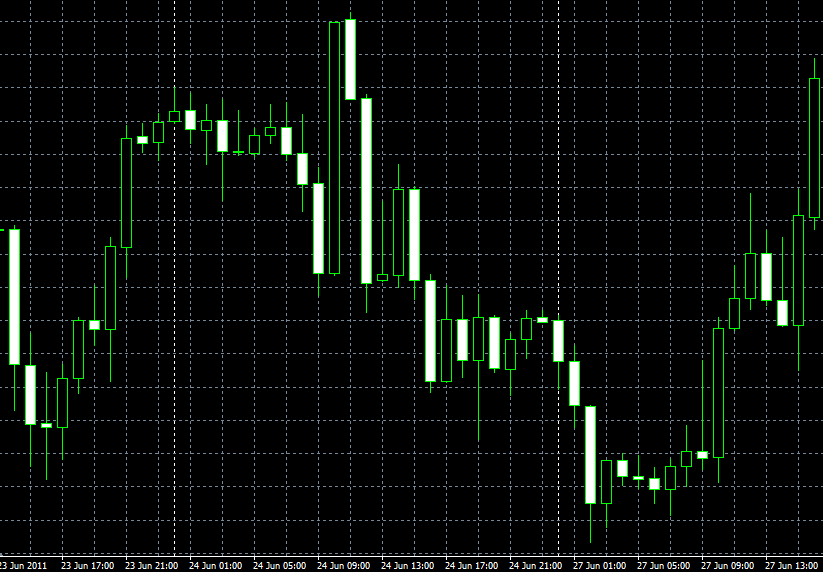
\includegraphics[width=15cm]{candles.png}
\caption{Wykres świecowy dla pary EUR/USD}
\label{swieca}
\end{center}
\end{figure} 
Poszczególne kształty świec mają odmienne znaczenia. Japończycy zdefiniowali różne rodzaje podstawowych świec oparte na relacjach między cenami otwarcia, zamknięcia, maksimami i minimami. Zbiór lub w niektórych przypadkach nawet pojedyncza świeca może tworzyć formację. Warto zaznaczyć, że taka formacja zwykle składa się z nie więcej niż pięciu świec. Większość formacji świecowych stosuje się do określania punktów zwrotnych na rynku, ale są też takie, które wskazują na kontynuację trendu. W analizie świecowej bardzo ważne jest zidentyfikowanie trendu, gdyż w zależności od jego kierunku istnieją różne formacje mówiące o jego odwróceniu. W przypadku japońskich świec, do rozpoznania trendu z powodzeniem stosuje się prostą średnią kroczącą, o krótkim okresie do 10 dni. Analiza świecowa najlepiej sprawdza się przy prognozach krótkookresowych, do 10 dni. W przeciwieństwie do wielu znanych metod nie podąża za trendem, lecz stara się wskazać momenty jego zwrotu. Wiecej informacji na temat formacji świec japońskich znajduję się w rozdziale \ref{swiece_rozdzial}.

Ostatnia metoda opiera sie na analizie wskaźników technicznych. Często potwierdzenia sygnałów płynących z analizy trendów i formacji poszukuje się we wskaźnikach technicznych. Istnieje wiele rodzajów wskaźników, z których każdy sprawdza sie lepiej w określonej sytuacji. Do prawidłowego zastosowania wskaźników potrzebna jest pewna wiedza na temat ich konstrukcji oraz sposobu interpretacji płynących z nich sygnałów. W niniejszej pracy wskaźniki techniczne odgrywać będą główną rolę. W kolejnych podrozdziałach zostaną przedstawione wskaźniki, które zostały użyte przy tworzeniu systemu do wspomagania decyzji na GPW. 
\section{Średnie ruchome}
\label{sec:srednie}
\paragraph{}
Średnie ruchome, inaczej zwane średnimi kroczącymi, są najczęściej stosowanymi narzędziami do budowy wskaźników technicznych. Łatwość obliczenia oraz jasność płynących z nich sygnałów sprawia, że stanowią one podstawę większości stosowanych systemów inwestycyjnych. Zasady dotyczące średnich kroczących w łatwy sposób można zaprogramować na komputerze, w przeciwieństwie do zasad analizy formacji, która jest w dużej części subiektywna i trudna do weryfikacji. 

Zasadą budowania prostej średniej kroczącej jest wyznaczenie średniej arytmetycznej z wybranej ilości okresów. Następnie do wyliczenia kolejnej wartości ,,przesuwamy się dalej'' tzn. bierzemy kolejną wartość, usuwając poprzednią i z otrzymanych danych ponownie wyliczamy średnią arytmetyczną. Istnieje wiele rodzajów średnich kroczących. Do najbardziej znanych można zaliczyć średnią prostą, średnią ważoną oraz średnią wykładniczą. Średnia prosta \textit{S(n,k)} w momencie 
\textit{n} z \textit{k} sesji (okresów) wyraża sie wzorem:
\begin{equation}
S(n,k)=\frac{1}{k}\sum_{i=n-k+1}^{n} P_{i}=\frac{1}{k}(P_{n-k+1}+P_{n-k+2}+...+P_{n})
\label{eqn:wzor}
\end{equation}
Średnia ważona \textit{SW(n,k)}:
\begin{equation}
SW(n,k)=\frac{1}{k}\sum_{i=n-k+1}^{n}w_iP_{i}
\label{eqn:wzor}
\end{equation}
zakładając, że wagi sumują się do 1 oraz są nieujemne:
\begin{equation}
\sum_{i=1}^{k}w_i=1, w_{i} \geq 0
\label{eqn:wzor}
\end{equation}
Średnia wykładnicza \textit{SWK(n,k)} wyraża się wzorem:
\begin{equation}
SWK(n,k)=rP_n+(1-r)SWK(n-1,k), SWK(1,k)=P_1
\label{eqn:wzor}
\end{equation}
gdzie \textit{r} oznacza procent wykładniczy i wynosi:
\begin{equation}
r=\frac{2}{k+1}
\label{eqn:wzor}
\end{equation}
\paragraph{}
Ilość okresów brana pod uwagę zależy od oczekiwanej długości naszej inwestycji. W analizie technicznej przyjęto podział na średnie krótkookresowe (5-20 sesyjne), średniookresowe (25-50 sesyjne) i długookresowe (50-100 sesyjne)\cite{8}. Dłuższe średnie np. 10- lub 13-tygodniowa, w połączeniu ze średnią 30- lub 40-tygodniową, były od dawana wykorzystywane w analizach rynków akcji, ale nie zwracano na nie większej uwagi w przypadku rynków terminowych. Średnie 10- i 30-tygodniowe można stosować w analizie głównych trendów widocznych na wykresach długoterminowaych Należy pamiętać, że średnie krótkookresowe często generują fałszywe sygnały sprzedaży, dlatego też zaleca się używać minimum 10 sesji do obliczania średniej. 

Jedną z wielkich korzyści płynących ze stosowania średnich kroczących i jedną z przyczyn popularności tego sposobu analizy trendu jest to, że realizuje on główne zasady prawidłowego dokonywania transakcji. Nakazują inwestować zgodnie z kierunkiem trendu, pozwalają na akumulację zysku i skłaniają do ograniczania strat. System analizy rynku oparty na średnich kroczących zmusza użytkownika do przestrzegania tych zasad, dostarczając określonych sygnałów kupna i sprzedaży. Średnie kroczące podążają za trendem, więc okazują się być najbardziej skuteczne wówczas, gdy istnieje wyraźny trend wzrostowy lub spadkowy. Natomiast słabo wypadają, gdy rynek znajduje się w trendzie horyzontalnym. Na niektórych rynkach podczas wyraźnego trendu średnie kroczące są najlepsze. W innych sytuacjach bardziej odpowiednie okazują się wskaźniki niezależne od istnienia trendu, takie jak oscylatory ukazujące wykupienie lub wyprzedanie rynku.
 
Najbardziej popularną zasadą w metodzie średnich kroczących, dotyczącą sygnału kupna jest przecięcie średniej od dołu przez cenę zamknięcia. Sygnał sprzedaży występuje przy przecięciu średniej od góry przez cenę zamknięcia. W analizie technicznej stosowane jest również podejmowanie decyzji za pomocą większej ilości średnich o różnych okresach. Ogólna zasada podejmowania decyzji w takim przypadku mówi, że sygnał kupna następuje, gdy dłuższa średnia (więcej okresów) zostaje przecięta od dołu przez krótszą średnia\cite{1}. Sygnał sprzedaży generuje przecięcie dłuższej średniej przez krótszą od góry.
\begin{figure}[ht]
\begin{center}
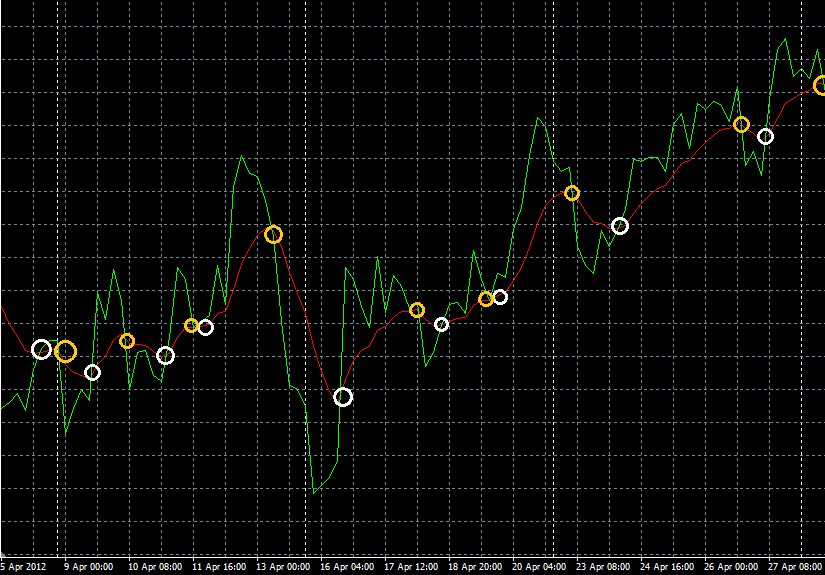
\includegraphics[width=15cm]{ma.png}
\caption{Wykres prostej średniej ruchomej z 10 okresów wraz z notowaniami pary EUR/USD}
\label{ma}
\end{center}
\end{figure}

Na rysunku \ref{ma} widać, że w dniach od 5 do 18 kwietnia, gdy trend nie jest do końca ukształtowany, prosta średnia ruchoma generuje sygnały nie przynoszące znaczących zysków. Dodatkowo często, są to sygnały mylne, które w dłuższym okresie przynoszą straty. Natomiast sygnał pojawiający się w czasie wyraźnego trendu wzrostowego, tworzącego się w okolicach 20 maja, daje okazję do osiągnięcia wysokiego zysku. W przypadku ukształtowania się trendu, istnieje mniej sygnałów ale są one o wiele bardziej wartościowe. Przytoczona sytuacja to jeden z przykładów na to, że średnie tego typu najlepiej sprawdzają się podczas wyraźnych trendów.

Jedną z popularnych metod podejmowania decyzji, opartej na prostej średniej kroczącej, jest metoda Wstęgi Bollingera. Nazwę zawdzięcza swojemu twórcy Johnowi Bollingerowi, amerykańskiemu analitykowi finansowemu, który prace nad wstęgami rozpoczął na początku lat 80, XX wieku. Wstęga powstaje przez narysowanie dwóch linii wzdłuż średniej ruchomej odległych o określoną ilość odchyleń standardowych, z dołu i z góry. Odchylenie standardowe to pojęcie statystyczne obrazujące rozproszenie wartości wokół średniej. Przyjmuje się, że średnią ruchomą wyznacza się z 20 sesji oraz odległość linii kontrolnych od niej ma wynieść 2 odchylenia standardowe. Przy zastosowaniu dwóch odchyleń standardowych, według panującej w statystyce reguły 2 sigm, 95 procent danych cenowych znajdzie się pomiędzy górną a dolną wstęgą\cite{5}. Odchylenie standardowe w metodzie Wstęg Bollingera jest obliczane w następujący sposób:
\begin{equation}
\sigma = \sqrt[2 ]{\frac{1}{k-1} \sum_{i=n-k+1}^{n}{[{P_{i}-S(n,k)}]}^{2} } 
\label{eqn:wzor}
\end{equation}

Wstęgi Bollingera cechują się dodatkową własnością. Wstęgi Bollingera rozszerzają się i zwężają w zależności od zmienności w okresie ostatnich 20 dni. W czasie rosnącej zmienności cen odległość pomiędzy dwiema wstęgami będzie się zwiększać, natomiast w okresach niskiej zmienności, odległość ta będzie sie zmniejszać. Kiedy wstęgi są od siebie oddalone dużo bardziej niż zwykle, jest to często oznaką końca trendu. Kiedy zaś odległość ta zbytnio się zmniejsza, może to oznaczać rychły początek nowego trendu\cite{5}. Wstęgi Bollingera można stosować także na wykresach długoterminowych, przyjmując zamiast 20 dni 20 tygodniu lub 20 miesięcy. Wstęgi te najlepiej sprawdzają się w połączeniu z oscylatorami wykupienia i wyprzedania. W metodzie tej sygnał kupna występuje, gdy cena jest bliska dolnej wstęgi, a sygnał sprzedaży, gdy cena zbliża się do wstęgi górnej. Silny sygnał kupna występuje dodatkowo jeśli średnia ruchoma, czyli wstęga środkowa, rośnie. Metoda ta ma zmienną skuteczność w zależności od aktualnego trendu.
\begin{figure}[ht]
\begin{center}
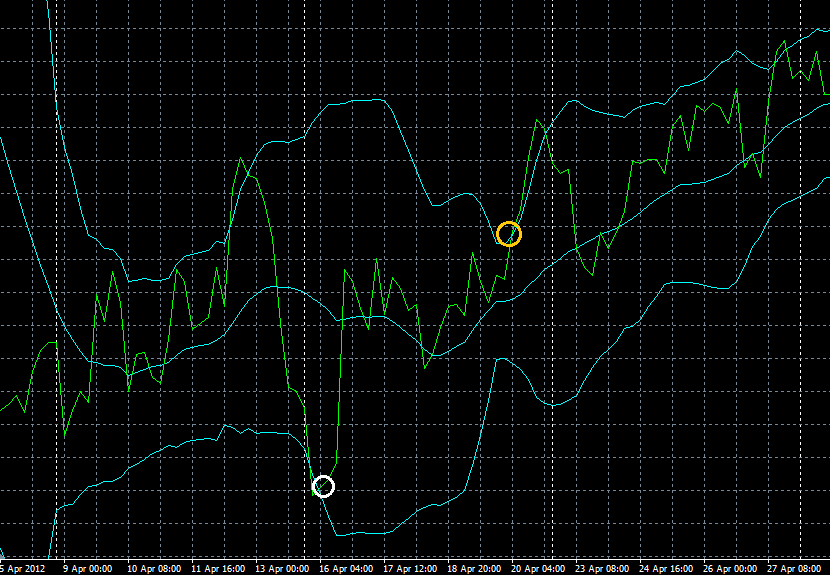
\includegraphics[width=15cm]{bb.png}
\caption{Wykres Wstęg Bollingera z 20 okresów wraz z notowaniami pary EUR/USD}
\label{bb}
\end{center}
\end{figure}
\paragraph{}
W przeciwieństwie do prostej średniej ruchomej, metoda Wstęg Bollingera generuje o wiele mniej sygnałów kupna i sprzedaży. W analizowanym okresie jest to jedna transakcja kupna, która przynosi wysokie zyski. Warto zwrócić uwagę, że w czasie trendu horyzontalnego, trwającego od 5 do 18 maja, ceny oscylują pomiędzy górną, a dolną wstęgą. W okresie znaczącego trendu wzrostowego, trwającego po 18 maja, ceny przebiegają jedynie pomiędzy górną a środkową linią. W czasie spadków, sytuacja odwraca się i cena oscyluje w granicach dolnej i środkowej linii. Do osiągnięcia lepszych wyników można wykorzystać ten fakt, ustawiając sygnały kupna na moment przecięcia środkowej linii przez ceny akcji, przy istnieniu wyraźnego trendu wzrostowego. Wstęgi Bollingera najlepiej sprawdzają sie w połączeniu z oscylatorami wykupienia i wyprzedania, które zostaną przedstawione w następnej części.
\section{Oscylatory}
\label{sec:oscylatory}
\paragraph{}
Alternatywę dla podejścia opartego na podejmowaniu decyzji zgodnie z trendem stanowią oscylatory. Użyteczność oscylatorów szczególnie widać na rynkach, gdzie nie występują wyraźne trendy. W sytuacjach takich większość systemów gry z trendem okazuje się po prostu mało skuteczna. Oscylatory stanowią zatem dla analityka narzędzie, dzięki któremu jest on w stanie osiągać zyski również w tych okresach, gdy na rynku nie ma wyraźnego trendu. Z badań wynika, że tylko około 30 procent czasu na rynku zajmuje wyraźny trend. Reszta czasu to horyzontalne wahania cen. Znaczenie oscylatorów nie ogranicza się jednak do okresów bocznych ruchów cen. Wykorzystywane w połączeniu z wykresami cen podczas trendów wzrostowych lub spadkowych oscylatory stają się źródłem niezwykle cennych sygnałów informujących o krótkoterminowych sytuacjach skrajnych, nazywanych powszechnie wykupieniem i wyprzedaniem rynku\cite{5}. Oscylator może również ostrzegać, że trend traci swój impet, zanim stanie się to widoczne w zachowaniach cen. Mogą też ukazywać różne dywergencje sygnalizujące, że pewien trend dobiega końca.

Oscylatory mają wiele wspólnych cech. Przypominają poziomą wstęgę umieszczoną pod wykresem cen. Mimo wzrostów, spadków lub bocznych ruchów kursów akcji, wstęga oscylatora biegnie poziomo. Osią oscylatora jest przeważnie poziom zerowy, dzielący go na górną i dolna część. John H. Murphy wyróżnił trzy najważniejsze zastosowania oscylatorów:
\begin{enumerate}
\item Oscylatory są najbardziej przydatne, kiedy osiągają skrajne wartości minimalne lub maksymalne. Mówi się, że rynek jest wykupiony, kiedy oscylator przebiega w pobliżu górnej granicy swoich wahań, zaś rynkiem wyprzedanym nazywa się sytuację, w której oscylator znajduje się w okolicach dolnego ekstremum. Stanowi to ostrzeżenie przed możliwością zmiany kierunku ruchu cen.
\item Dywergencja, czyli rozbieżność pomiędzy zachowaniem oscylatora i ruchem cen w sytuacji, gdy oscylator znajduje się blisko swojego ekstremum, jest zazwyczaj istotnym ostrzeżeniem przed możliwością zmiany trendu.
\item Przecięcie poziomu zerowego może stanowić ważny sygnał do zawierania transakcji zgodnych z kierunkiem głównego trendu.
\end{enumerate}

MACD to jeden z oscylatorów, skonstruowany na podstawie średnich wykładniczych. Metoda MACD (ang. \textit{moving averages convergence, divergence}) została opracowana przez G. Appel’a. Narzędzie to jest bardzo użyteczne, ponieważ łączy w sobie pewne zasady dotyczące oscylatorów z metodą przecięcia dwóch średnich. W swojej pierwotnej wersji metoda MACD sugeruje posłużenie się średnimi wykładniczymi 26-tygodniową i 12-tygodniową, których różnica zostaje wygładzona za pomocą średniej wykładniczej 9-tygodniowej. Jednak na każdym z rynków występują różne odmiany opisywanej metody. W Polsce najpopularniejszym sposobem jest stosowanie 17-dniowej i 8-dniowej średniej wykładniczej\cite{1}. Różnica tych średnich jest nazywana linią MACD. Linia MACD, wygładzona średnią wykładniczą 9-dniową nazywana jest linią sygnału. W metodzie MACD można znaleźć kilka sposobów na generowanie sygnałów. Główna zasada, sprawdzająca się przy analizie średnich, mówi o tym, że sygnał kupna występuje przy przecięciu od dołu dłuższej średniej przez krótszą. Sygnał sprzedaży występuje, gdy średnia krótsza przebija od góry średnią dłuższą. Na wykresie MACD kupno i sprzedaż są zauważalne odpowiednio, gdy linia MACD przecina od dołu poziom 0 oraz gdy przecina od góry poziom 0. Można tu również obserwować dywergencje pomiędzy liniami MACD i ceną. Negatywna dywergencja występuje wówczas, gdy linie MACD znajdują sę wyraźnie powyżej poziomu zerowego (wykupienie) i zaczynają słabnąc, a ceny nadal rosną. Często jest to ostrzeżenie, że formuje się szczyt cenowy. Pozytywna dywergencja pojawia się, gdy linie MACD są wyraźnie poniżej poziomu zero (wyprzedanie) i zaczynają rosnąc, wyprzedzając ceny. Jest to często wczesny sygnał informujący, że ukształtowało się dno cenowe. Dla rozpoznawania istotnych zmian trendu można na wykresie MACD wytyczać linie trendu.

Dodatkowe informacje o sygnałach kupna i sprzedaży można wyciągać z analizy wzajemnego położenia linii MACD oraz linii sygnału. Za pomocą różnicy między tymi dwoma średnimi kroczącymi konstruuje się histogram. W przypadku metody MACD składa się on z pionowych słupków, które pokazują różnicę pomiędzy dwiema liniami MACD. Ponownie ich wzajemne położenie będzie sugerować pewne decyzje. Gdy różnica między linią MACD, a linią sygnału przetnie od dołu poziom 0 należy spodziewać się wzrostu cen, a przecięcie od góry linii 0 sugeruje zbliżający się spadek kursów akcji. Główną zaletą histogramu jest możliwość określenia, kiedy rozstęp między dwiema liniami zwiększa się lub zmniejsza. Jeśli histogram przebiega powyżej swojego poziomu zerowego, ale zaczyna spadać ku niemu, to trend wzrostowy słabnie. I na odwrót, jeśli histogram znajduje się poniżej swojego poziomu zerowego, ale zaczyna rosnąc ku niemu, to trend spadkowy traci impet. Dopóki histogram nie przetnie swojego poziomu zerowego, nie ma jeszcze sygnałów kupna lub sprzedaży, ale te zmiany kierunku są wczesnymi ostrzeżeniami, że aktualny trend słabnie. Zwroty histogramu ku linii zero można wykorzystywać jako wczesne sygnały do zamykania pozycji. Dużo bardziej niebiezpieczne byłoby stosowanie ich jako sygnałów do otwierania nowych pozycji przeciw dominującemu trendowi. Przypadek w którym linia MACD i histogram przecinają od dołu poziom zero jest najpewniejszym sygnałem kupna, a dodatkowo wzrost średnich wykładniczych 17 i 8-dniowych daje silny sygnał kupna\cite{1}. Silny sygnał sprzedaży analogicznie generowany jest przy spadku obu średnich wykładniczych wraz ze spełnieniem obu wcześniejszych warunków. 

Podobnie jak w przypadku wszystkich wskaźników technicznych sygnały na wykresach sporządzanych w ujęciu tygodniowym są bardziej istotne od sygnałów występujących na wykresach dziennych. Najlepszym sposobem ich wykorzystywania jest stosowanie sygnałów tygodniowych do określania kierunku trendu, a sygnałów dziennych do sprecyzowania momentu zawarcia transakcji. Sygnał krótkoterminowy jest ważny tylko wówczas, gdy zgadza się z sygnałem długoteminowym. W ten oto sposób sygnały długoteminowe stają się filtrami dla sygnałów krótkoterminowych i zapobiegają dokonywaniu transakcji przeciw dominującemu trendowi\cite{5}.
\begin{figure}[ht]
\begin{center}
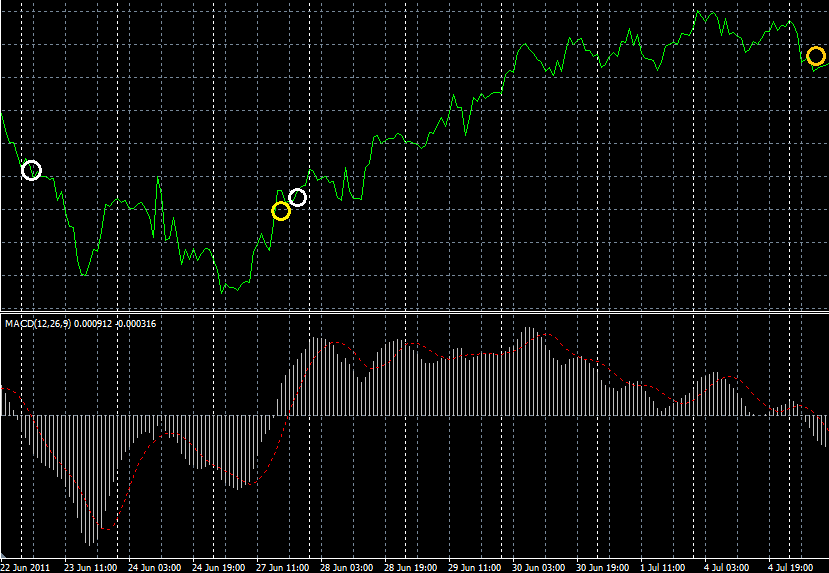
\includegraphics[width=15cm]{macd.png}
\caption{Wykres oscylatora MACD(26,12,9) wraz z notowaniami pary EUR/USD}
\label{macd}
\end{center}
\end{figure}

Poniżej przedstawiono przykład interpretacji wskaźnika MACD. Notowania pary EUR/USD w przedstawionym okresie czasu początkowo charakteryzowały się trendem horyzontalnym. Następnie kurs skoczył do góry przyjmując stały trend wzrostowy. Metoda MACD wygenerowała wartościowe sygnały w obu przypadkach, które pozwoliłyby inwestorowi osiągnąć zyski. Sygnały te zostały stworzone, analizując jedynie przebieg linii MACD. Użycie dodatkowo różnicy linii MACD z linią sygnału w niektórych przypadkach daje o wiele większe zyski. Pierwszym z sygnałów jest zajęcie pozycji krótkiej sprzedaży na początku 22 czerwca. Wtedy linia MACD przecina od góry poziom 0. Zamknięcie pozycji następuje w połowie 27 czerwca. Pomimo trendu horyzontalnego, w którym cięzko przewidzieć ruchu cenowe, transakcja została zakończona niewielkim zyskiem. Po zamknięciu pozycji, powinna zostać otwarta pozycja kupna. Wyraźnie widać, że taki ruch okazałby się trafną decyzją gdyż zamknięcie kupna nastąpiłoby dopiero pod koniec 4 lipca z wyraźnym zyskiem. Dodatkowo opierając się na histogramie dzien 23 czerwca można uznać za moment wyprzedania i otworzyć pozycję długą (kupna). Za punkt wykupienia w tym przypadku mógłby posłużyć poziom osiągnięty pod koniec 27 czerwca. Również w ten sposób zostałaby zrealizowana zyskowna transakcja. Jak widać, wskaźnik MACD podlega wielu interpretacjom, które w określonych przypadkach przynoszą różne efekty. 
\section{Formacje świec japońskich}
\label{swiece_rozdzial}
\paragraph{}
Zadaniem japońskich technik analizy wykresów jest rozpoznawanie odpowiednich formacji składających się z jednej lub kilku świec. Każda z formacji posiada zdefiniowaną budowę oraz warunki występowania. Niestety informacje te nie zawierają ścisłych wytycznych przez co ich interpretacja podlega subiektywnym ocenom. Mimo tego, technika analizy świec japońskich staje się coraz bardziej popularna wśród zachodnich inwestorów. Metoda ta swoje uznanie zawdziecza możliwości obserwacji psychologii graczy, powodującej podejmowanie okreśłonych decyzcji na rynku. Emocje inwestorów takie jak strach, nadzieja czy chciwość mają bezpośredni wpływ na rynkową sytuację. Giełda Forex jako największy rynek, na którym dzienne obroty sięgają bilionów dolarów, nie ulega wpływom ,,wielkich'' graczy. Rynek ten to ciągła walka podaży i popytu większości inwestorów. Dlatego, też poznanie psychologii podejmowania decyzji przez ,,tłum'' stanowi klucz do osiągania sukcesów. Klucz ten, odzwierciedlający zachowanie graczy w okreśłonych momentach, znajduje się w poszczególnych formacjach świec japońskich. 

Formacje można podzielić na trzy rodzaje. Pierwszym z nich są te które zapowiadają trend wzrostowy. Posiadają one swoje odpowiedniki w formacjach prognozujących spadki. Do ostatniej kategori należą formację kontynuacji trendu. W pracy tej zostaną omówione jedynie szablony świec znajdujące się w punktach zmiany trendu. Każda z formacji składa się w większości z jednej do pięciu świec. Już te składające się z pojedyńczych świec dają wiele informacji na temat runku. W wielu przypadkach są to sygnały o wiele bardziej wartościowe od tych płynących z bardziej rozbudowanych sekwencji świec. Jest to spowodowane możliwością ich prostszego identyfikowania na wykresie przez większą grupę inwestorów, co w oczywisty sposób wpływa na psychologie podjęcia konkretnej decyzji. 

W metodzie świec japońskich istnieje powiązanie pomiędzy poszczególnymi typami formacji. Dla wzorców zapowiadających hosse istnieją odpowiednie formacje prognozujące spadki. Również dla formacji bardziej złożonych można znaleźć pojedyńcze świece, które im odpowiadają. Takie powiązania można wychwycić wybierając na wykresie okres prezentowanych danych, gdzie kolejne świece zmieniają swój przedział czasowy, który opisują. Do najpopularniejszych okresów przedstawiania danych należą przedziały 1-minutowe, 15-minutowe, 30-minutowe, godzinne, 4-godzinne, dzienne i tygodniowe. Z tego wynika, że na wykresie świeca 15-minutowa składa się z piętnastu świec 1-minutowych. Dlatego, też istnieje metoda pozwalająca na redukcję formacji skłądających się z kilku świeć do świec pojedyńczych. Żeby utworzyć korpus nowej świecy należ wybrać cenę otwarcia pierwszej oraz cenę zamknięcia świecy ostatniej. Na rysunku \ref{redukcja} cena otwarcia święcy pierwszej znajduje się u góry jej korpusu, ze względu na spadkowy charakter. Cena zamkniecia świecy białej, oznaczającej wzrost, występuje w tym wypadku również w górnej części korpusu. Po uzyskaniu korpusu nowej świecy należy określić jeszcze cene maksymalną oraz minimalną. W tym celu wybiera się cene maksymalną i minimalną z całej redukowanej formacji. W przypadku rysunku \ref{redukcja} będą to skrajne ceny ostatniej świecy. Zredukowana formacja ma tę samą wymowę co bardziej złożona sekwencja świec. 
\begin{figure}[ht]
\begin{center}
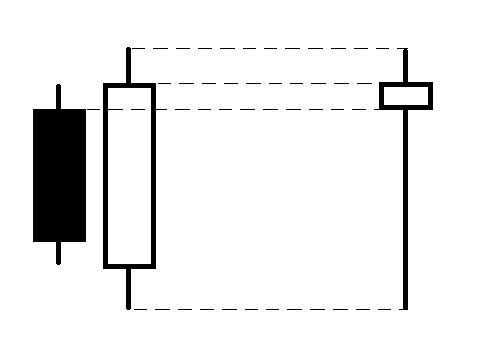
\includegraphics[width=10cm]{reduction.png}
\caption{Redukowanie formacji do świecy pojedyńczej}
\label{redukcja}
\end{center}
\end{figure} 

Formacji skłądających się z pojedyńczych świec istnieje stosunkowo niewiele wśród wszystkich opisanych w publikacjach o japońskich technikach analizy wykresów. Mimo to są to wzorce dobrze odzwierciedlające aktualną sytuacje na rynku. Do najpopularniejszych formacji tego typu należą ,,młot'' i ,,wisielec''. 
\begin{figure}[ht]
\begin{center}
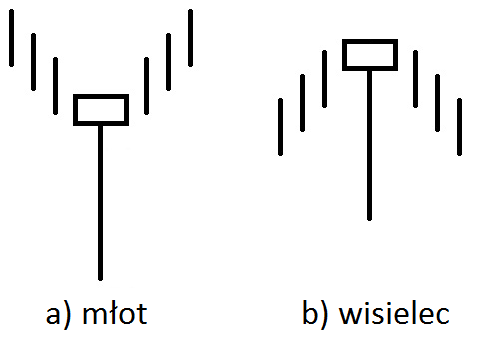
\includegraphics[width=10cm]{hammer.png}
\caption{Budowa formacji a) młota i b) wisielca}
\label{mlot}
\end{center}
\end{figure} 

Obie składają się z pojedyńczej swiecy. Posiadają długi dolny cień i małe korpusy, które znajduja sie na poziomie lub w pobliżu maksymalnego dziennego zasięgu zmian kursu. Co oznacza, że cień górny nie występuje lub jest bardzo krótki. Kolor korpusu świec nie jest aż tak istotny w przypadku tych formacji ze względu na jego nieduża wielkość.

Formacja młota występuje w trendzie spadkowy i zapowiada trend wzrostowy. Stąd też bierze się jej nazwa, gdyż tak jak młot spada i odbija się ku górze. Moment kształtowania się formacji zaczyna się gdy rynek znajduje się w trendzie spadkowym. Wśród inwestorów dominuje wtedy nastawienei negatywne. Kolejne otwarcie następuje na pewnym poziomie, po czym kurs gwałtowanie spada. Jednakże ma miejsce osłabienia wyprzdaży i kurs powraca do maksymalnej ceny osiągniętej w czasie danej sesji lub w jej pobliżu. Nieudana próba kontynuacji trendu spadkowego w znacznym stopniu zmniejsza negatywne nastawienie rynku, a większość inwestorów posiadających pozycje krótkie znajdzie się w kłopotliwej sytuacji. Jeśli kurs zamknięcia znajduje się powyżej kursu otwarcia, powodując utworzenie się świecy w kolorze białym, sytuacja staje się jeszcze bardziej korzystna dla byków. Potwierdzeniem tej formacji będzie otwrcie na wyższym poziomie podczas kolejnej sesji, wraz z jeszcze wyższym zamknięciem.  

Formacja wisielca występuje w czasie trwania trendu wzrostowego, a dokładnie w jego szczytowym momencie. Swoją nazwę wisielec zawdzięcza wyglądowi świecy, przypominającej wiszącego człowieka. W czasie tworzenia się formacji wisielca rynek uważany jest za rynek byka, gdyż od pewnego czasu trwa trend wzrostowy. Aby formacja wisielca mogła się ukształtować, kurs w czasie trwania sesji musi znacznie spaść z poziomu otwarcia, a następnie powrócić i zamknąć się w pobliżu maksymalnych wartości. Powoduje to utworzenie się długiego dolnego cienia, który wskazuje, że na rynku może rozpocząć się wyprzedaż. Jeśli podczas kolejnej sesji rynek otwiera się na niższym poziomie, może okazać się, że na rynku jest wielu inwestorów posiadających długie pozycje, którzy będą szukali okazji do sprzedaży. Potwierdzeniem spadkowej wymowy formacji wisielca może być czarny kolor korpusu oraz otwarcie na niższym poziomie podczas kolejnej sesji.

Kolejnymi przykładami formacji jednoświecowych są ,,odwrócony młot'' oraz ,,spadająca gwiazda''. Obie posiadają pojedyńczą swiecę o niewielkim korpusie. Cień dolny praktycznie nie występuje, za to górny kilkakrotnie przewyższa długością korpus. Wymowa tych świec jest słabsza, niż młota i wisielca, dlatego niezbędne jest potwierdzenie.  
\begin{figure}[ht]
\begin{center}
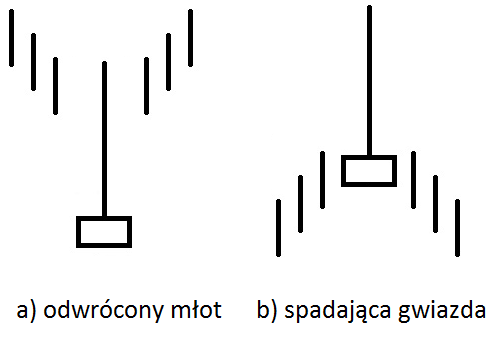
\includegraphics[width=10cm]{invert_hammer.png}
\caption{Budowa formacji a) odwróconego młota i b) spadającej gwiazdy}
\label{odwr_mlot}
\end{center}
\end{figure} 

Podobnie jak formacja pokrewna - młot, formacja odwróconego młota pojawia się w trendzie spadkowym i sugeruje możliwość zmiany kierunku trendu. Momentem rozpoczęcia tworzenie się omawianej świecy w trendzie zniżkującym jest otwarcie na niższym poziomie, powodujące utworzenie się luki cenowej w stosunko do świecy poprzedniej. Wzrostom, które pojawiają się w ciągu sesji, nie udaje się utrzymać i rynek zamyka się w pobliżu swojego minimum. Podobnie jak w przypadku formacji młota oraz formacji wisielca, poziom otwarcia kolejnej sesji ma kluczowe znaczenie dla sukcesu lub porażki formacji odwróconego młota jako zwiastuna zmiany kierunku trendu. Jeśli więc kolejnego dnia otwarcie następuje powyżej korpusu odwróconego młota, pojawienie się możliwości odwrócenia trendu spowoduje zamykanie przez inwestorów krótkich pozycji, co z kolei umocni trend wzrostowy. Odwrócony młot może łatwo stać się częścią formacji porannej gwiazdy, mającej jeszcze mocniejszą wzrostową wymowę. 

Spadająca gwiazda skłąda sie z pojedyńczej świecy, wskazującej na możliwość zakończenia trendu wzrostowego. Nie jest to jednak mocny sygnał odwrócenia. Formacja spadającej gwiazdy wygląda dokładnie tak samo jak formacja odwróconego młota. Różnicą jest oczywiście to, że spadająca gwiazda występuje w trendzie wzrostowym. W czasie trwania trendu następuje otwarcie na wyższym poziomie powodując utworzenie się luki cenowej. Następnie kurs osiąga kolejne maksima, lecz zamknięcie następuje w pobliżu minimum. Takie zachowanie, w obliczu utworzonej luki cenowej, ma jednoznacznie negatywną wymowę. Spowoduje też oczywiście pewne zaniepokojenie wszyskich ,,byków'' posiadających zyski na pozycjach. 
 
Nieco bardziej rozbudownym przykładem formacji jest ,,objęcie''. Składa się ona z dwóch świec posiadających korpusy w odmiennych kolorach. Korpus drugiej świecy całkowicie obejmuje korpus świecy z dnia poprzedniego. W przypadku tej formacji cienie nie są brane pod uwagę. Gdy formacja ta wystapu w pobliżu szczytu, wskazuje na zmianę nastawienia rynku w kierunku sprzedaży. Formacja objęcia hossy może zostac zredukowana do postaci młota. Objęcie bessy zostaje zredykowane do formacji zbliżonej do spadającej gwiazdy. 
\begin{figure}[ht]
\begin{center}
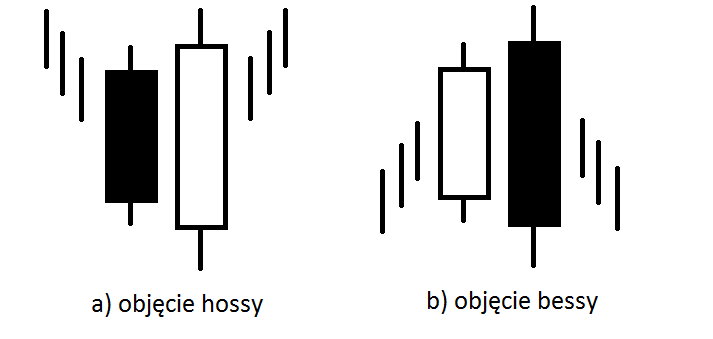
\includegraphics[width=10cm]{engulfing.png}
\caption{Budowa formacji a) objęcia hossy i b) objęcia bessy}
\label{objecie}
\end{center}
\end{figure} 

Pierwsza ze świec, utworzona w formacji objęcia, posiada niewielki korpus, podczas gdy druga ma wysoki korpus własny. Ponieważ druga utworzona świeca jest o wiele bardziej wymowna, odzwierciedla ona możliwość zakończenia dotychczasowego trendu. Jeśli formacja objęcia o wymowie spadkowej pojawia się po długotrwałym wzroście, znacznie zwiększa ona prawdopodobieństwo, że większość byków zajęła już pozycje długie na rynku. W tym przypadku może nie wystarczyc nawet duży kapitał, aby utrzymać trwający trend wzrostowy.

W czasie tworzenia się formacji objęcia bessy trwa trend wzrostowy. Pojawia się świeca z niedużym białym korpusem przy niewielkim obrocie. Podczas kolejnej sesji kurs otwiera sie na nowym maksymalnym poziomie, a następnie szybko spada. Spadek odbywa się przy dużym wolumenie obrotów, a kurs zamknięcia następuje poniżej poziomu otwarcia z dnia poprzedniego. Intuicyjnie można stwierdzić, iż trend wzrostowy został powstrzymany. Jeśli podczas kolejnej sesji kurs pozostanie na niższym poziomie, będzie to jednoznacznym potwierdzeniem zmiany ytrendu. Całkowicie przeciwny scenariusz będzie miał miejsce dla formacji objęcia hossy.

Pokrewną formacją do ,,objęcia'' jest ,,harami''. Składa się ona z przeciwstawnie ułożonych świec. Wymagane jest, aby korpus drugiej świecy został całkowicie objęty przez korpus świecy utworzeonej podczas poprzedniej sesji. 
\begin{figure}[ht]
\begin{center}
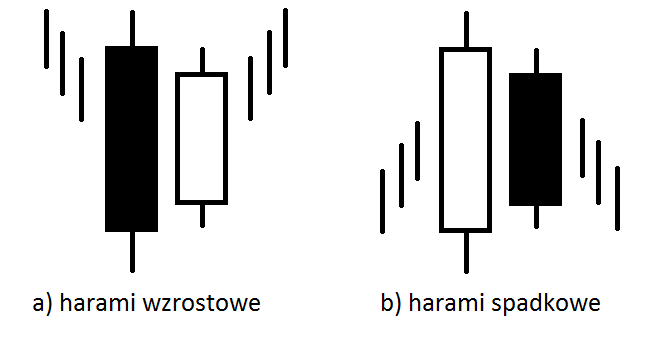
\includegraphics[width=10cm]{harami.png}
\caption{Budowa formacji a) harami wzrostowe i b) harami spadkowe}
\label{harami}
\end{center}
\end{figure} 

Formacja harami wzrostowego pojawia się w trakcie trwania trendu zniżkowego. Tworzy sie wysoka czarna świeca przy średnim poziomie obrotów, która umacnia spadkowe nastawienie rynku. W czasie kolejnej sesji otwarcie następuje na wyższym poziomie, co zaskakuje graczy posiadających krótkie pozycje. Wiele z nich zostaje zamkniętych, powodując dalszy wzrost kursu. Zostaje on jednak ograniczony przez spóźnialskich inwestorów, którzy wykorzystują sytuację do dokonania krótkiej sprzedaży, czego nie zdążyli zrobić poprzednim razem. Wolumen obrotów na tej sesji przekracza ich poziom z dnia poprzedniego, co sugeruje masowe pokrywanie pozycji krótkich. Potwierdzenie odwrócenia na trzeciej sesji dostarczy potrzebnego dowodu na to, że nastąpiła zmiana kierunku trendu.

W trakcie tworzenia się harami spadkowego trwa trend rosnący, który zostaje potwierdzony utworzeniem się wysokiej białej świecy oraz dużym wolumenem obrotów. W czasie kolejnej sesji otwarcie następuje po niższym kursie i nie zmienia sie w sposób znaczący przez całą sesję. Zamknięcie ma miejsce na nieco niższym poziomie, lecz ciągle wewnątrz korpusu świecy utworzonej w dniu poprzedni, W obliczu tak gwałtownego załamania się trendu inwestorzy krótkoterminowi powinni zastanowić sie nad siłą rynku, szczególnie gdy wolumen obrotów jest niewielki. Jednoznacznie wskazuje to, iz trend może niedługo zmienić kierunek. Potwierdzeniem będzie niższy poziom zamknięcia kolejnej, trzeciej sesji. Tak jak formacje objęcia harami może być zredukowane do młota i spadającej gwiazdy. 

Kolejną popularną formacją skłądającą się z dwóch swieć jest ,,przenikanie''. Jej przeciwieństwem jest ,,zasłona ciemnej chmury''. Formacja przenikania występuje w trendzie spadkowym rynku. Pierwsza ze świec ma kolor czarny i podtrzymuje trend spadkowy, świeca druga natomiast posiada wysoki biały korpus, w którym otwarcie następuje na poziomie nowego minimum, ale zamknięcie ma miejsce powyżej połowy korpusu świecy utworzonej w dniu poprzednim. 
\begin{figure}[ht]
\begin{center}
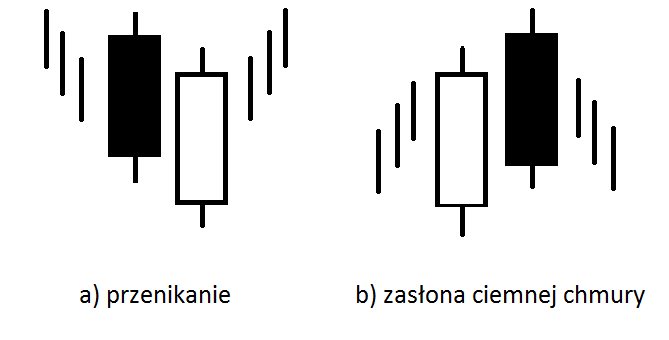
\includegraphics[width=10cm]{piercing.png}
\caption{Budowa formacji a) przenikanie i b) zasłona ciemnej chmury}
\label{przenikanie}
\end{center}
\end{figure} 

Pierwsza wysoka czarna świeca formacji, występująca w trendzie spadkowym, podtrzymuje zniżkową wymowę rynku. Luka spadkowa utworzona na otwarciu kolejnej sesji dodatkowo umania trend zniżkowy. Jednakże rynek wzrasta przez całą sesję i zamyka się na znacznie wyższym poziomie. Zamknięcie to znajduje sie powyżej połowy korpusu wysokiej czarnej świecy utworzonej w dniu poprzednim. Taka sytuacja wywołuje zaniepokojenie wśród ,,niedźwiedzi'' i przyczynia się do uformowania potencjalnego dna. Wykresy świecowe doskonale ilustrują taka właśnie sytuację, podczas gdy wykresy słupkowe ledwo ją odnotowują. Formacja przenikania może zostać zredukowana do postaci młota.  

Zasłona ciemnej chmury jest formacja odwórcenia hossy. Ponieważ formacja ta występuje tylko w trendzie wzrostowym, pierwsza świeca ma wysoki biały korpus, który odzwierciedla kierunek trendu. Otwarcie kolejnego dnia następuje powyżej maksimum białej świecy z dnia poprzedniego. Jest to jeden z nielicznych przypadków. kiedy maksimum czy minimum śa wykorzystywane przy definiowaniu formacji świecowych. Spadek kursu w ciągu całego dnia powoduje, że zamknięcie nastepuje poniżej połowy wysokiej białej świecy. 

Przy trendzie wzrostowym tworzy się typowa wysoka biała świeca. Podczas kolejnej sesji rynek otwiera się na wyższym poziomie, powodując utworzenie się luki cenowej, lecz jest to już ostatnio wzrost, na jaki stać rynek ,,byka''. Zaczynają się spadki aż do momentu zamknięcia, które następuje wewnątrz korpusu białej swiecy z poprzedniego dnia, lecz poniżej jej środka. Każdy inwestor, który uważał rynek za wzrostowy, z pewnościa przemyśli w takim momencie swoja strategię inwestycyjną. Podobnie jak w przypadku formacji przenikania, mamy do czynienia z jednoznacznym odwróceniem trendu.
 
Ostatnimi najbardziej rozbudowanymi formacjami opisywanymi w pracy są gwiazda poranna i gwiazda wieczorna. 
\begin{figure}[ht]
\begin{center}
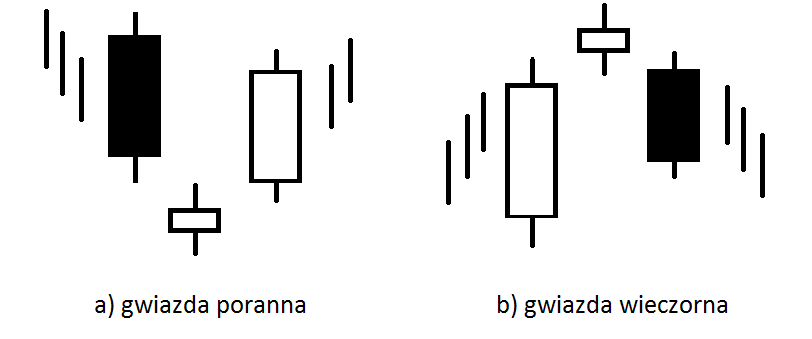
\includegraphics[width=12cm]{stars.png}
\caption{Budowa formacji a) gwiazdy porannej i b) gwiazdy wieczornej}
\label{gwiazdy}
\end{center}
\end{figure} 

Gwiazda poranna jest formacją odwrócenia bessy. Jej nazwa wskazuje, że przewiduje ona możliwość pojawienia się wyższych cen. Składa się z wysokiej czarnej świecy, po której pojawia sie luka spadkowa oraz świeca o niewielkim korpusie. Trzecia świeca ma biały korpus, który zachodzi na korpus czarny świecy pierwszej. Optymalna formacja gwiazdy porannej będzie posiadała lukę cenową zarówno przed, jak i po środkowej świecy formacji.

Przy kształtowaniu się gwiazdy porannej trwa trend spadkowy. Pojawia się charakterystyczna dla tego trendu wysoka czarna świeca. Otwarcie kolejnej sesji następuje na niższym poziomie, po luce cenowej. Zakres zmian cen jest niewielki, a zamknięcie następuje na poziomie zbliżonym do poziomu otwarcia. Utworzony niewielki korpus wskazuje na początek niezdecydowania na rynku. Otwarcie kolejnej sesji ma miejsce nieco wyżej, po utworzeniu się luki cenowej, a zamknięcie następuje na jeszcze wyższym poziomie. Nastąpiło jednoznaczne odwrócenie trendu. W przypadku formacji gwiazdy wieczornej scenariusz wydarzeń stanowi przeciwieństwo sytuacji zachodzących przy gwieździe porannej.

Formacją o przeciwnej do gwiazdy porannej wymowie jest formacja gwiazdy wieczornej. Ponieważ gwiazda wieczorna jest formacja zapowiadającą spadek, występuje ona w trendzie wzrostowym. Pierwsza świeca ma wysoki biały korpus, po którym pojawia sie gwiazda. Korpus gwiazdy jest oddzielony luka cenową od korpusu poprzedniej świecy. Niewielka świeca w postaci gwiazdy jest pierwszym znakiem pojawienia sie niezdecydowania na rynku. Trzecia świeca występuje na niższym poziomie, po luce cenowej, co kończy kształtowanie się tej formacji. Podobnnie jak gwiazda poranna, formacja gwiazdy wieczornej powinna posiadać luki cenowe pomiędzy korpusami pierwszej i drugiej świecy oraz pomiędzy korpusami świecy drugiej i trzeciej.

Przedstawione przykłady świec japońskich stanowią niewielki odsetek formacji opisywanych w literaturze. Jednak należą do najpopularniejszych sekwencji świec, a tym samym są najwnikliwiej analizowane i najczęściej wykorzystywane. Nie są to formacje szczególnie rozbudowane. Ograniczona ilość kryteriów definujących przedstawione świece daje możliwość dosyć prostego rozpoznania danej formacji. Wpływa na to fakt, że subiektywizm przy klasyfikacji danej sekwencji świec do odpowiedniego szablonu jest mniejszy dla formacji prostszych. Dzięki temu mniej rozbudowane formacje są częściej zauważane na rynku, a tym samym ich wymowa jest bardziej wiarygodna. Mniejszy zakres kryteriów daje szanse na stworzenie skuteczniejszych systemów rozpoznających daną formację.  
 
\section{Systemy transakcyjne}
\paragraph{}
W analizie technicznej komputer odgrywa coraz większą rolę. Należy podkreślić, że jest niezwykle cennym narzędziem w rękach tego, kto zna podstawy analizy technicznej. Jeśli nie ma się włąściwej znajomości koncepcji, jakie leżą u podstaw rozmaitych wskaźników i nie zna się sposobów ich interpretacji, można zagubić się w gąszczu dostępnych dziś programów komputerowych\cite{8}.

Na rynku istnieje wiele rozbudowanych systemów służących do analiz technicznych. Do najpopularniejszych należą MetaTrader, MetaStock, Amibroker, TradeStation, WealthLabl. Jednak najdynamiczniej rozwijającym się oprogramowaniem, z którego korzysta coraz większa ilość inwestorów, jest MetaTrader, stworzony przez firmę MetaQuotes Software Corp
\begin{figure}[ht]
\begin{center}
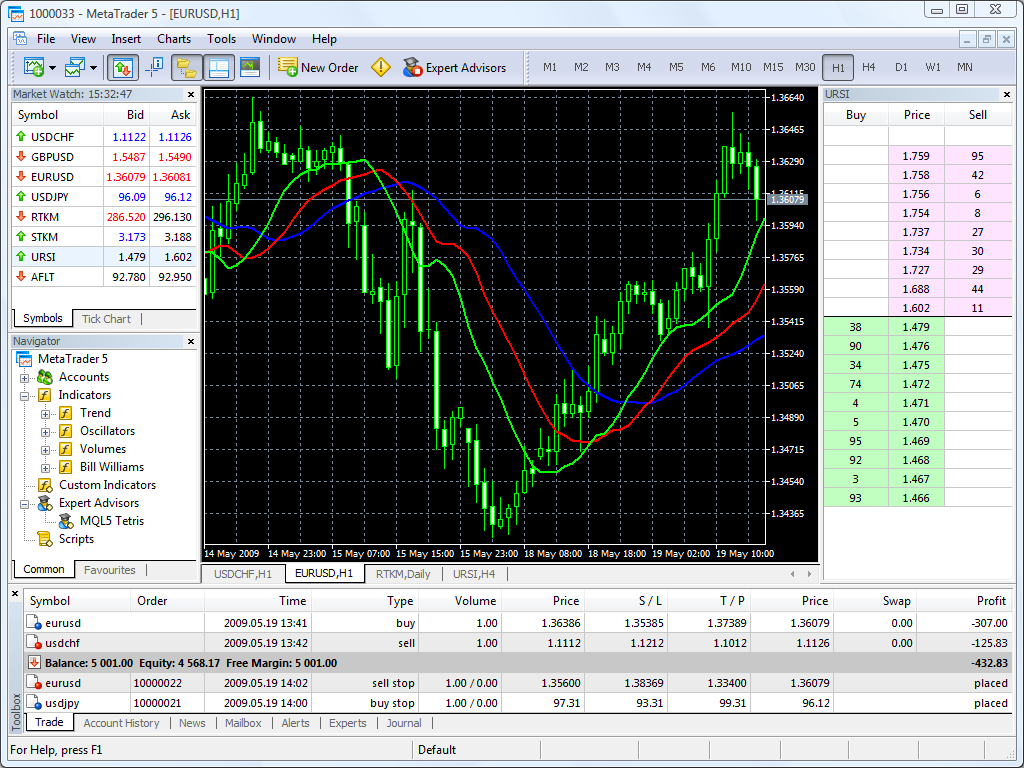
\includegraphics[width=15cm]{metatrader.png}
\caption{Zrzut ekranu z programu MetaTrader}
\label{swieca2}
\end{center}
\end{figure} 
MetaTrader to nowoczesna platforma handlu internetowego zaprojektowana w celu zapewnienia usług maklerskich dla klientów na rynkach Forex, CFD, Futures. System MetaTrader składa się z wielu modułow przeznaczonych dla brokerów oraz graczy giełdowych. Każdy z elementów systemu odpowiada za konkretną funkcjonalność. Wspólnie tworzą system w pełni pokrywający potrzeby klientów. Platforma składa się z sześciu głównych modułów.
 \begin{enumerate}
\item MetaTrader Serwer - to serce systemu, w którym są przetwarzane wszystkie transakcje handlowe. Odpowiada za przechowywanie i zarządzanie danymi historycznymi.
\item MetaTrader Administrator - umożliwia zdalną administrację serwerem. Umożliwia przygotowanie instrumentów finansowych oraz zarzadzania bazą danych.
\item MetaTrader Centrum danych - to serwer proxy który ma na celu zwiększenie skalowalności i bezpieczeństwa plarformy.
\item MetaTrader Terminal klienta - to narzędzie, które umożliwia graczowi przeprowadzanie analizy technicznej, dokonowanie transakcji handlowych i korzystania z wielu innych udogodnień
\item MetaTrader Terminal mobilny - umożliwia zarządzanie kontem i analizę techniczną dla graczy posiadających urządzenia przenośne.
\end{enumerate}

Z punktu widzenia brokera MetaTrader oferuje możwliość łatwego i wydajnego zarządzania grupą klientów, instrumentów finansowych, baz danych i wiele innych. Graczom giełdowym oferuje niespotykana w innych programach liczba wskaźników, wykresów, gotowych strategii i analiz. Oprócz tego charakteryzuje się wysoką szybkością pracy oraz współpracą z pakietem Microsoft Office. Umożliwia tworzenie wskaźników oraz strategii inwestycyjnych przy użyciu własnego języka programowania mql. Istnieje możliwość testowania zarówno dostępnych strategii, jak i stworzonych samodzielnie. W aplikacji zaimplementowano moduł szukający najlepszych inwestycji przy zadanych kryteriach. Po uporządkowaniu dokonuje klasyfikacji otrzymanych wyników. Dzięki temu inwestor może skupić się na tych walorach, które w danej sytuacji pozwalają na osiągnięcie największego zysku. Dodatkowo system oferuje moduł do nauki. Polega on na podejmowaniu decyzji na danych historycznych i sprawdzaniu ich faktycznego zachowania w przyszłości.

Nie ma wątpliwości, że komputer zrewolucjonizował analizę rynków finansowych i świat transakcji. Programy komputerowe pozwalają łączyć analize techniczną z analizą fundamentalną. Wielką korzyścią wynikającą z posługiwania się komputerem jest możliwość uczenia się dzieki programom do analizy rynku. Podręczniki użytkownika mają nierzadko rozmiary pokaźnych ksiąg i zawierają wszelkiego rodzaju wyjaśnienia oraz wzory. Zdolności komputera do dawania sygnałów ostrzegawczych są szczególnie pomocne dla tych, którzy obserwują rynki akcji i obligacji na całym świecie oraz tysiące poszczególnych spółek. Algorytmy inwestycyjne tworzone w ramach systemów posiadają szereg zalet:
\begin{enumerate}
\item Eliminowane są emocje.
\item Osiąga się większą dyscyplinę.
\item Możliwa staje się większa konsekwencja.
\item Transakcje są dokonywane zgodnie z kierunkiem trendu.
\item Praktycznie gwarantowane jest uczestnictwo w każdym istotnym trendzie.
\item Zyski mogą rosnąć.
\item Straty są minimalizowane.
\end{enumerate}

Niestety większość z nich cechuje kilka wad:
\begin{enumerate}
\item Większość systemów mechanicznych podąża za trendem.
\item Systemy podążające za trendem potrzebują wyraźnych trendów, aby przynosic zyski.
\item Systemy zależne od trendu nie przynoszą na ogół zysków, kiedy na rynku nie ma wyraźnego trendu.
\item Okresy bez wyraźnych trendów bywają bardzo długie, co utrudnia stosowanie tego podejścia.
\end{enumerate}

\chapter{Projekt systemu}
\label{chap:projekt}
\paragraph{}
W poprzednich rozdziałach pracy przedstawione zostały teoretyczne zasady analizy technicznej. Dzięki właściwemu stosowaniu prezentowanych metod można osiągać wymierne korzyści na rynkach finansowych. Opierając się na tychże zasadach istnieje możliwość skonstruowania efektywnego automatycznego systemu inwestycyjnego. Oprócz przynoszenia zysków tego typu system stawia wiele innych wymagań, które zostaną przedstawione w dalszej części rozdziału wraz ze sposobem realizacji projektu.

\section{Określenie wymagań i założeń projektu}
\paragraph{}

Opisywany automatyczny system inwestycyjny stawia szereg wymogów. Głównym zadaniem tworzonego algorytmu jest zdolność do przeprowadzania transakcji na rynku Forex przy minimalnej ingerencji gracza. Użytkownik oprócz wyboru waluty na której będzie działał system, powinien mieć możliwość jedynie zmiany podstawowych parametrów działania programu przed jego uruchomieniem. Oczywiście tego typu system powinien zapewniać zyski przy jednoczesnej ochronie kapitału gracza. Na użytkowniku powinna spoczywać decyzja co do stopnia ryzyka przeprowadzanych inwestycji. W trakcie ciągłej pracy aplikacji, może pojawiać się wiele wyjątków, które zakłócą działanie systemu. Każdy z nich musi być obsłużony. Jeśli to możliwe, po wystąpieniu takiej sytuacji, powinna zostać wznowiona praca programu. W innym wypadku działanie aplikacji powinno zostać natychmiast przerwane, a użytkownik poinformowany o zaistniałym zdarzeniu. Dodatkowo inne istotne sytuacje powinny zostać zaraportowane i udostępnione użytkownikowi.  

Projekt systemu został opracowany przy uwzględnieniu kilku założeń. Algorytm dostosowano do najpopularniejszej pary walutowej EUR/USD. Oznacza to, że wszystkie domyślne parametry zostały zoptymalizowane pod kątem tego instrumentu. Mimo to, sprawdzają się również na innych parach walutowych. W celu dopasowania ustawień użyte zostały dane historyczne z różnych okresów. Analizie poddano świece 15-miutowe. W celu prostszego testowania strategii, w każdym momencie działania programu, dopuszcza się istnienie jedynie jednej otwartej pozycji. Do stworzenia algorytmów została użyta platforma Metatrader 4 wraz z językiem mql4. Testy przeprowadzono na koncie demo największego polskiego brokera XTB. 

W dalszej części pracy zostaną zaprezentowane diagramy UML obrazujące funkcjonalność systemu, sposób działania zaimplementowanych algorytmów oraz interakcje z innymi systemami.



\section{Diagramy UML}
\paragraph{}

\subsection{Diagramy przypadków użycia}
\paragraph{}

\begin{figure}[H]
\begin{center}
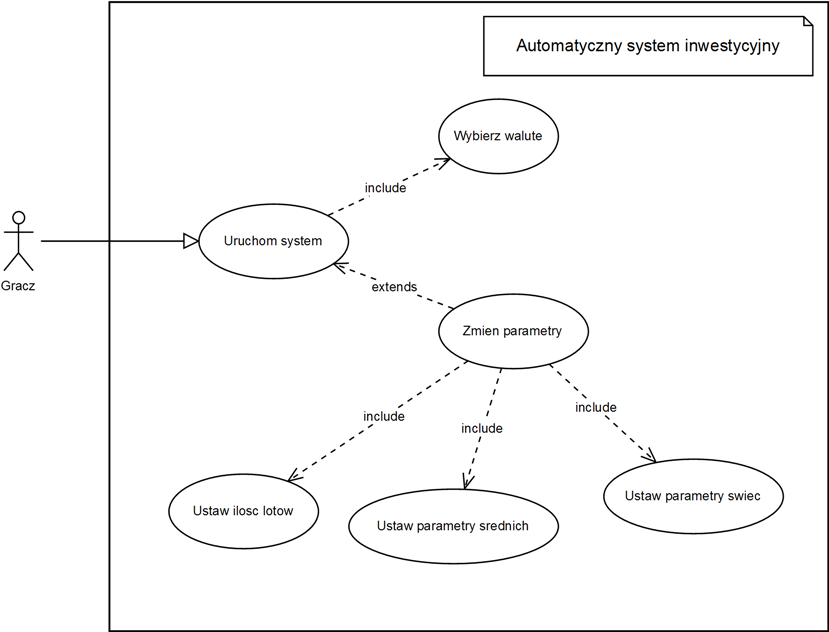
\includegraphics[width=16cm]{usecase.PNG}
\caption{Diagram przypadków użycia}
\label{usecase}
\end{center}
\end{figure} 

\begin{itemize}
\item
Gracz - aktor użytkownik uruchamiający automatyczny system inwestycyjny na wybranej parze walutowej. Ma możliwość zmiany ustawień przy starcie aplikacji. 
\item
Uruchom system - Uruchomienie algorytmu na wybranej parze walutowej.
\item
Wybierz walutę - Wybranie waluty, spośród oferowanych przez brokera, na której ma działać algorytm. 
\item
Zmień parametry - Zmiana parametrów działania algorytmu.
\item
Ustaw ilość lotów - Ustawienie parametru odpowiedzialnego za ryzyko inwestycji gracza. Szczegółowe informacje na temat tego parametru znajdują się w części teoretycznej \ref{sec:forex}.
\item
Ustaw parametry średnich - Ustawienie parametrów średnich wykładniczych odpowiedzialnych za rozpoznawanie trendów.
\item
Ustaw parametry świec - Ustawienie parametrów odpowiedzialnych za rozpoznawanie danej formacji świecowej.
\end{itemize}

\subsection{Diagramy aktywności}
\paragraph{}

\begin{figure}[H]
\begin{center}
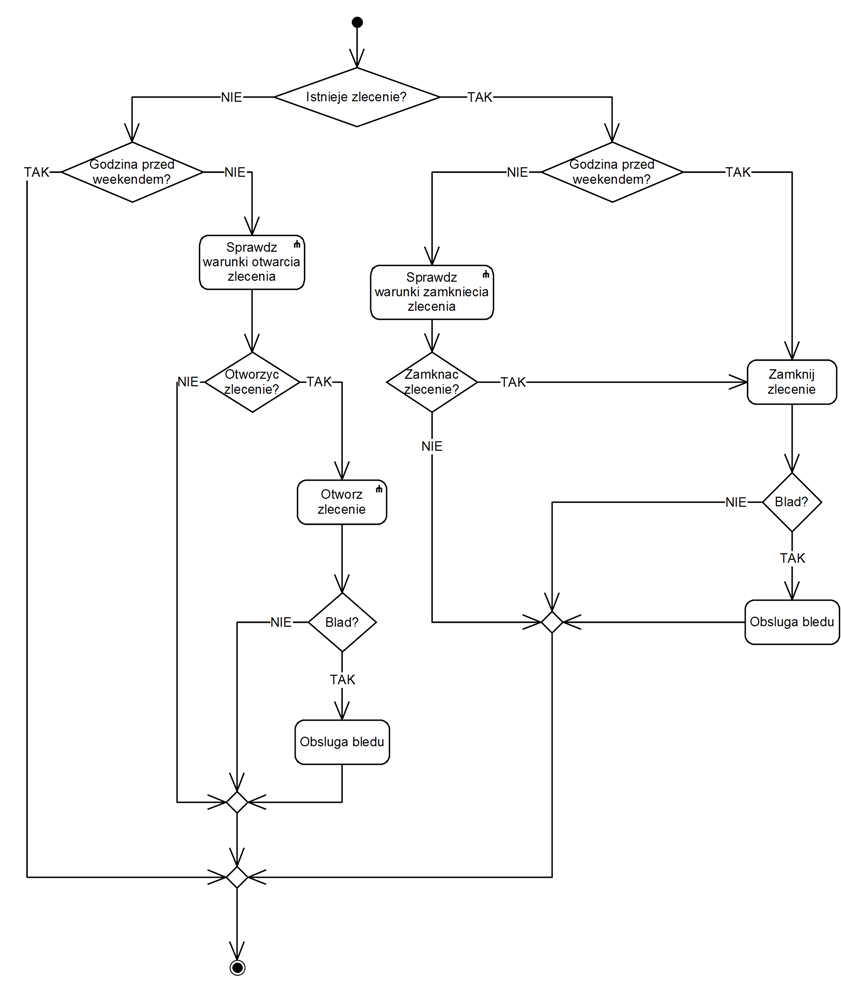
\includegraphics[width=16cm]{ogolny.png}
\caption{Diagram przedstawiający ogólny algorytm działania systemu}
\label{ogolny}
\end{center}
\end{figure} 

Diagram \ref{ogolny} obrazuje ogólny algorytm przeprowadzania transakcji w systemie. Przedstawiona procedura zostaje uruchomiona każdorazowo po pojawieniu się nowej świecy 15-minutowej. Program obsługuje jedynie jedno zlecenie w danym momencie. Dlatego, jeśli zlecenie jest otwarte sprawdzane są warunki zamknięcia pozycji. W przeciwnym razie sprawdzana jest możliwość złożenia zlecenia zakupu, bądź sprzedaży. Ze względu na fakt, że rynek Forex nie działa w weekendy, zamykane są pozycje, które chwile przed końcem sesji piątkowej są nadal otwarte. Dodatkowo w tym czasie nie przeprowadzane są inne transakcje. Takie postępowanie, chroni gracza przed ewentualną utratą kapitału po wystąpieniu luki cenowej. Zjawisko to opisane jest dokładniej w rozdziale \ref{sec:forex}. Przy wystąpieniu sygnału kupna, bądź sprzedaży zostaje wysłane żądanie otwarcia danej pozycji. W tym momencie następuje obsłużenie ewentualnych błędów. 

\begin{figure}[H]
\begin{center}
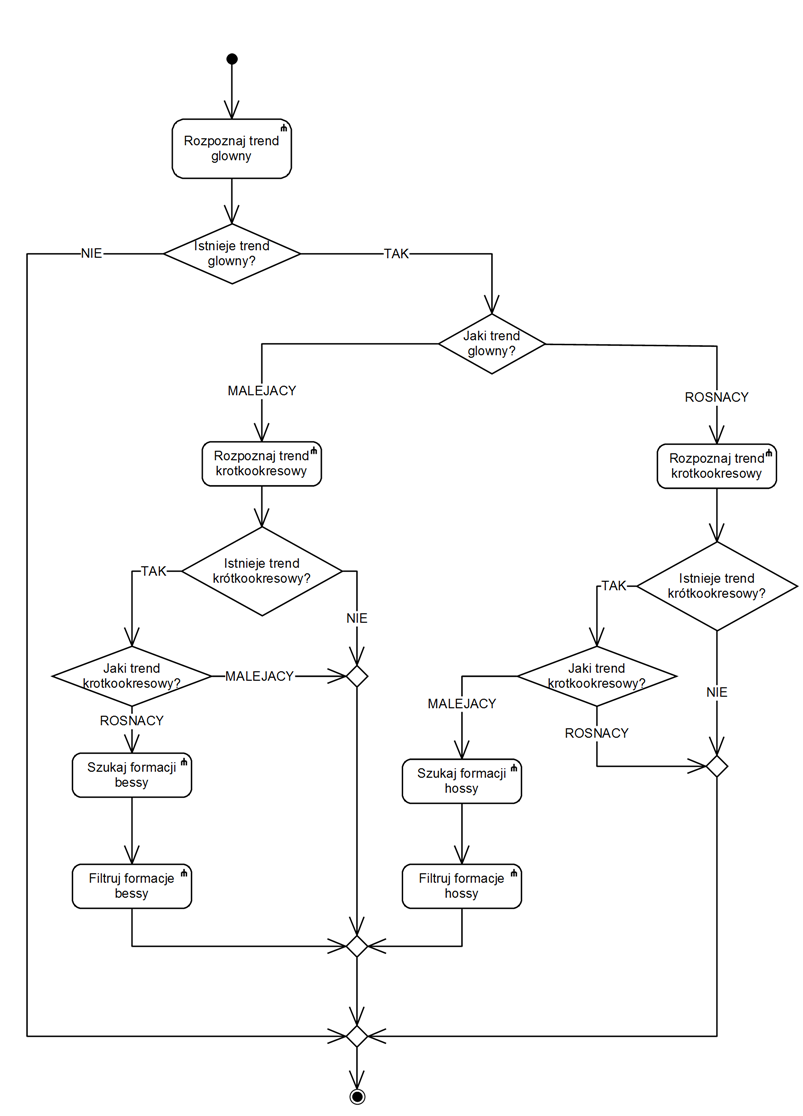
\includegraphics[width=16cm]{warunki_otwarcia.png}
\caption{Diagram przedstawiający algorytm poszukiwania formacji}
\label{warunki_otwarcia}
\end{center}
\end{figure} 

Na diagramie \ref{warunki_otwarcia} przedstawiono sposób generowania sygnałów kupna, bądź sprzedaży. Znalezienie konkretnej formacji nie może być podstawą do podejmowania decyzji na rynku. Oprócz zidentyfikowania określonej sekwencji świec, należy również przeanalizować miejsce, w którym dana formacja się znajduje. Przedstawiony algorytm opiera się na wyszukiwaniu świec w miejscach korekt rynku. Dlatego, też elementami algorytmu są fazy rozpoznania trendów długoterminowego i krótkoterminowego. Trend dłuższy oznaczać będzie główny kierunek rynku, w którym zawierane będą transakcje. Natomiast trend krótszy używany będzie do zlokalizowania korekt trendu długoterminowego. Oczekiwaną sytuacją będzie, moment w którym trend długoterminowy będzie w kierunku przeciwnym do trendu krótkoterminowego. W tych miejscach poszukiwane będą formacje odwrócenia trendu prognozujące zmianę trendu którkookresowego w kierunku trendu głównego. 

%\begin{figure}[ht]
%\begin{center}
%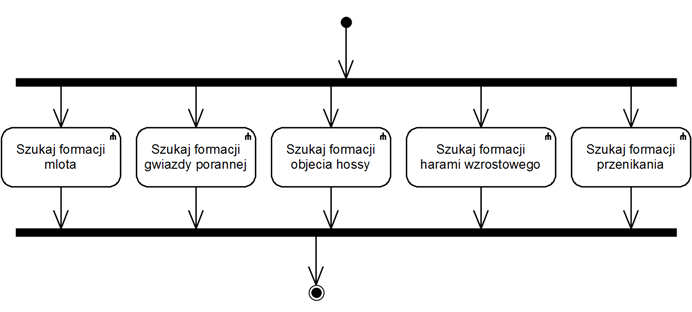
\includegraphics[width=12cm]{formacje_hossy.png}
%\caption{Diagram przedstawiający ogólny algorytm rozpoznawania dostępnych formacji hossy}
%\label{hossy}
%\end{center}
%\end{figure} 

Poszukiwanie formacji hossy lub bessy, w algorytmie z diagramu \ref{warunki_otwarcia}, opiera się na próbie znalezienia sekwencji świeć, pasującej do grupy obsługiwanych przez program wzorców. W przypadku analizy formacji hossy odpowiedni fragment kodu wywołuje się w momencie wystąpienia trendu głównego o kierunku wzrostowym wraz z krótkookresowym trendem malejącym. Opisywana część algorytmu dzieli się na szukanie formacji:
\begin{enumerate}
\item młota
\item gwiazdy polarnej
\item objęcia hossy
\item harami wzrostowego
\item przenikania
\end{enumerate}

Proces znajdowania formacji bessy uruchamiany jest w momencie znalezienia rosnącego trendu krótkookresowego przy malejącym trendzie głównym. Poszukiwane formacje to:
\begin{enumerate}
\item wisielec
\item spadająca gwiazda
\item objęcia bessy
\item harami spadkowe
\item zasłona ciemnej chmury
\end{enumerate}

Problem subiektywizmu, przy klasyfikacji danego zbioru świec do odpowiedniego wzorca, uniemożliwia zdefiniowanie jednoznacznych wytycznych opisujących konkretną formację. Każdy z przedstawionych warunków w rozdziale \ref{swiece_rozdzial}, w którym opisanywany jest wygląd poszczególnych sekwencji świec, daje pewien zakres dowolnej interpretacji. 

\begin{figure}[H]
\begin{center}
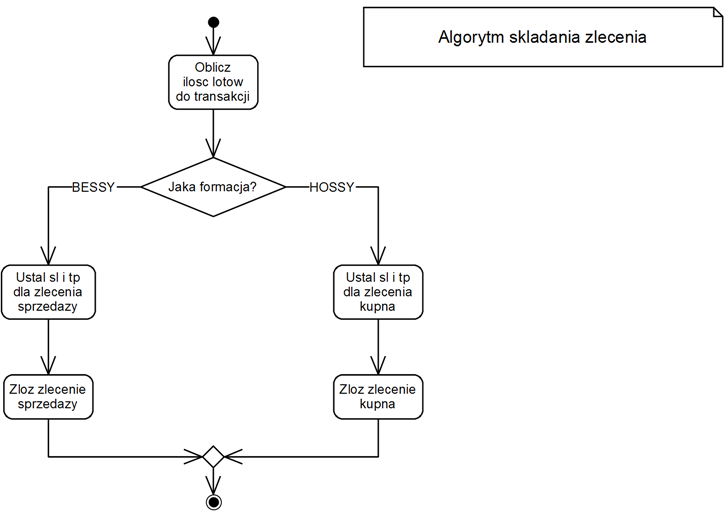
\includegraphics[width=12cm]{otwarcie.png}
\caption{Diagram przedstawiający algorytm otwierania zlecenia}
\label{otwarcie}
\end{center}
\end{figure} 

Powyższy diagram objaśnia proces składania zlecenia kupna, bądź sprzedaży. Jeśli przed uruchomieniem systemu użytkownik nie poda ilości lotów do transakcji, zostanie ona automatycznie obliczona jako wartość maksymalna. Takie postępowanie zwiększa ryzyko zawieranych transakcji. Jego ograniczeniem będzie ustawienie zarówno limitów stop loss jak i take profit. Sposób określenia limitów oraz typ transakcji będzie się różnić w zależności od tego czy wcześniej wystąpiła formacja hossy czy bessy, . Dla większości rozpoznawanych formacji pułap stop loss będzie ustawiany na krańcową wartość. W przypadku formacji hossy będzie to minimalna cena z całej formacji, a w formacji bessy wartość maksymalna. Zamykanie transakcji będzie opierać się głównie na oddzielnym algorytmie, dlatego pułap take profit ustawiany będzie na stałą wartość. Przy wystąpieniu formacji hossy wysyłane będzie zlecenie kupna, a zlecenie sprzedaży podczas znalezienia formacji bessy.   

\subsection{Diagramy sekwencjii}
\paragraph{}

\begin{figure}[H]
\begin{center}
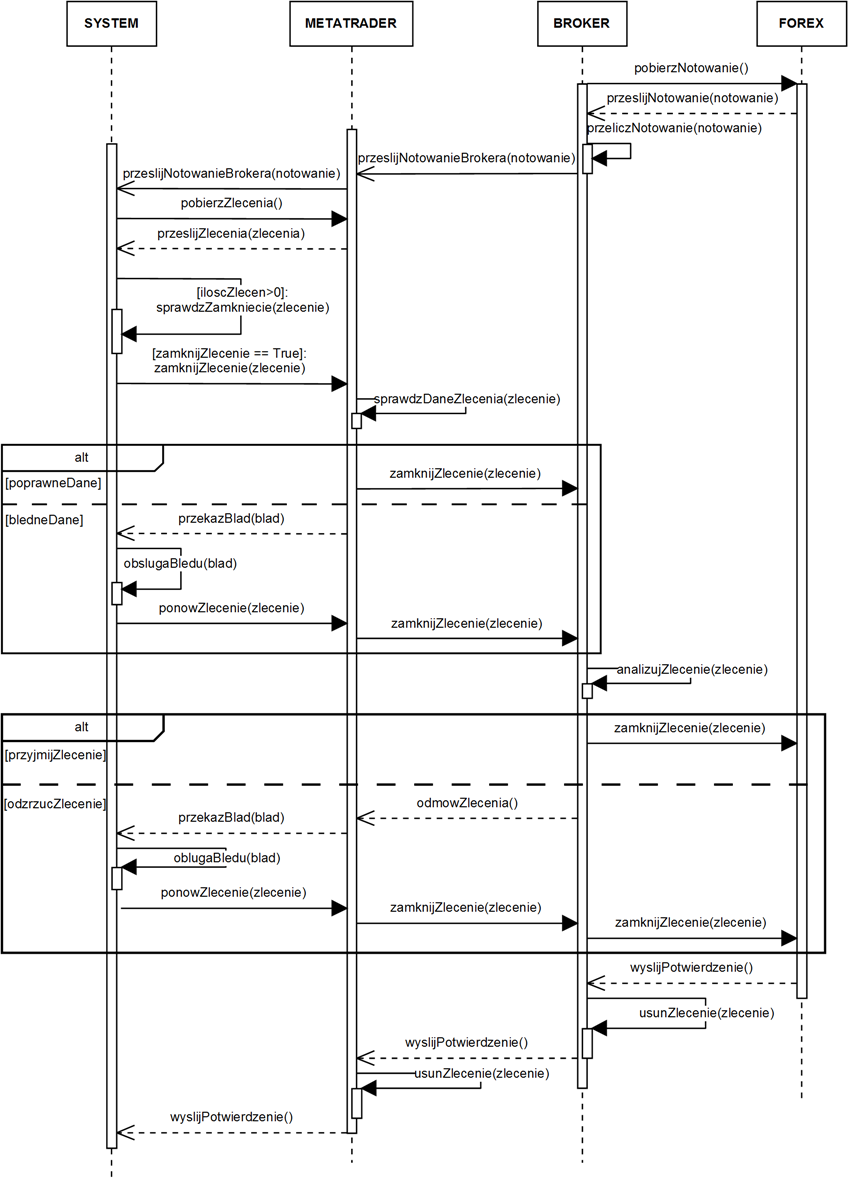
\includegraphics[width=16cm]{sekwencji.png}
\caption{Diagram opisujący interakcje pomiędzy częściami systemu}
\label{sekwencji}
\end{center}
\end{figure} 

Na diagramie \ref{sekwencji} został przedstawiony sposób komunikacji pomiędzy zaimplementowanym algorytmem, a systemami, które uczestniczą w czasie działania programu. Wyszczególnione zostały komunikaty, pojawiające się podczas procesu zamykania zlecenia. Do podejmowania decyzji na rynku Forex niezbędne są aktualne notowania. Najnowsze dane są pobierane przez brokerów bezpośrednio z rynku Forex. Jednak nie są one natychmiast przekazywane do klientów. Broker, po analizie aktualnie otwartych pozycji, może zmienić dane notowanie. Po przeanalizowaniu danych oraz ewentualnej korekcie, notowanie trafia do platformy inwestycyjnej. Aplikacja kliencka odpytuje co pewien czas serwer brokera w celu pobrania aktualnie dostępnych danych. Algorytm uruchomiony na platformie odczytuje wcześniej pobrane notowanie. Opisywany system analizuje każdą, nowo przychodzącą, daną. W pierwszym etapie sprawdzana jest ilość otwartych zleceń. Dane o zleceniach są przechowywane zarówno przez platformę inwestycyjną jak i system brokera. Algorytm poddaje analizie istniejące zlecenia. W przypadku decyzji o zamknięciu pozycji wysyłana jest odpowiednia informacja do MetaTrader'a wraz z niezbędnymi danymi. Platforma sprawdza poprawność przesłanych danych i w przypadku braku błędów wysyła żądanie zamknięcia pozycji do brokera. Wystąpienie błędu powoduje przesłanie sterowania do algorytmu wraz z komunikatem o błędzie. Błąd zostaje obsłużony, po czym następuje ponowienie akcji zamknięcia zlecenia. Żądanie zostaje dalej przekazane z platformy handlowej do systemu brokera. Tam poddawane jest analizie przez system brokerski. W przypadku akceptacji zlecenie zostaje ostatecznie zamknięte. Przesyłane są komunikaty zwrotne do każdego z systemów oraz odświeżane informacje o obecnych pozycjach. Informacja o ewentualnie pojawiającym się błędzie zostaje przekazana, aż do algorytmu inwestycyjnego, gdzie następuje obsługa oraz ponowne wykonanie akcji.

\section{Algorytmy rozpoznawania formacji świec japońskich}
\paragraph{}

W podrozdziale zostanie przedstawiony sposób w jaki identyfikowane będą poszczególne formacje świec japońskich. Opierając się na informacjach teoretycznych zawartych w rozdziale \ref{swiece_rozdzial}, zostały stworzone algorytmy realizujące kolejne reguły. 

Najważniejszym elementem przy klasyfikacji świec do odpowiedniego wzorca jest poprawne rozpoznanie trendu. Często miejsce wystąpienia formacji w odniesieniu do aktualnego trendu decyduje o tym czy mamy do czynienia z formacja hossy czy bessy.  Miejscami szczególnymi, w których wyszukiwane będą szablony świec japońskich są obszary korekt trendów głównych. Według diagramu \ref{warunki_otwarcia} w takich punktach można wyznaczyć trend główny oraz trend krótkookresowy. Wystąpienie w tym momencie formacji odwrócenia może świadczyć o końcu korekty i powrocie notowań do trendu głównego. Ewentualne decyzje o transakcji będą zgodne z głównym trendem na rynku.

Trend długookresowy, oznaczający trend główny, wyznaczono za pomocą przecięcia dwóch średnich wykładniczych. Ten sposób rozpoznawania trendu cieszy się duża popularnością wśród inwestorów i z powodzeniem sprawdza się na wielu rynkach.  Algorytm polega na odjęciu od siebie dwóch średnich wykładniczych z różnych okresów. Średnia biorąca pod uwagę mniej okresów odpowiada trendowi krótkookresowemu. Od niej odejmowana jest wartość średniej biorącej pod uwagę większą ilość notowań historycznych. Ilości okresów obu średnich to dwie zmienne, które należy odpowiednio dobrać w drodze optymalizacji. Dodatkowo w celu wykluczenia pomyłek przy trendach horyzontalnych, został wprowadzony parametr, który określa poziom oddalenia dwóch średnich. Jeśli wartość różnicy jest wystarczająco większa od 0 trend uznawany jest za rosnący. Wartości bliskie 0 to trend horyzontalny, w trakcie którego nie są podejmowane decyzje o kupnie, bądź sprzedaży. Wynik odpowiednio mniejszy od 0 mówi o pojawieniu się trendu spadkowego. 

Po rozpoznaniu trendu głównego poszukiwany jest moment w którym występuje korekta notowań. Do tego celu została użyta metoda Wstęg Bollingera omówiona w rozdziale \ref{sec:srednie}. Chwilowe odwrócenie rynku sygnalizowane jest pojawieniem się trendu krótkookresowego. Wstęgi Bollingera, opierając się na założeniach średnich kroczących, często używane są do identyfikowania zmian trendu. W metodzie używane są dwa parametry. Pierwszy z nich określa ilość okresów branych pod uwagę przy wyznaczaniu średniej kroczącej, która wyznacza środkową wstęgę. Drugi parametr oznacza o ile odchyleń standardowych odległe są wstęgi skrajne od wstęgi środkowej. Te dwie wartości można poddawać optymalizacji jednak na rynkach najczęściej używa się 20 okresów oraz 2 odchyleń standardowych. 

\begin{figure}[h!]
\begin{center}
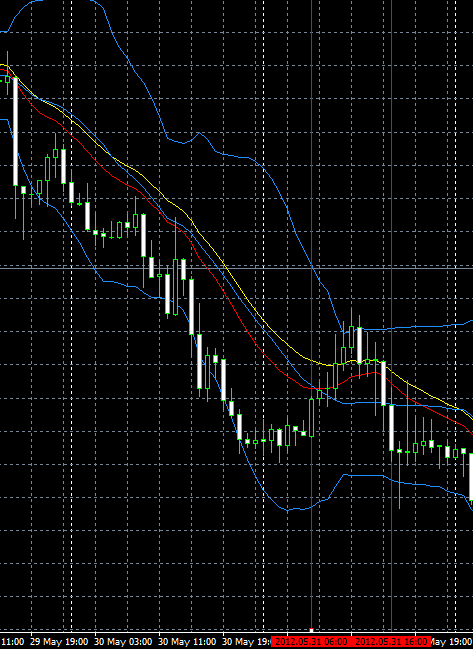
\includegraphics[width=12cm]{trend.png}
\caption{Wykres przedstawiający proces rozpoznawania korekty na rynku}
\label{trend}
\end{center}
\end{figure} 

W przypadku istnienia trendu głównego linia notowań znajduje się blisko skrajnych Wstęg Bollingera. Początek korekty występuje w sytuacji gdy wstęga środkowa zostaje przecięta przez notowania. W momencie gdy ceny oscylują pomiędzy środkową, a skrajną wstęgą wyszukiwane są formacje świec. Sytuacja taka została przedstawiona na wykresie \ref{trend}. Linie czerwona i żółta oznaczają odpowiednio średnią wykładniczą krótszą oraz dłuższą. Położenie średniej krótszej poniżej średniej dłuższej, wskazuje na występowanie spadkowego trendu długookresowego. Niebieskie linie to wstęgi bollingera. Obszar pomiędzy pionowymi czerwonymi liniami wskazuje miejsce korekty trendu. W takim miejscu poszukiwane są formacje świec zapowiadające koniec korekty i powrót do trendu głównego. Będą to formacje odwrócenia trendu prognozujące kolejne spadki. Sekwencje świec zwiastujące wzrosty będą występować przy rosnącym trendzie głównym oraz oscylacji notowań pomiędzy środkową, a dolną wstęgą bollingera.  

Kolejność rozpoznawania formacji zależy od sprawdzalności sygnałów z niej płynących. Świece, które w danym momencie najlepiej prognozują przyszłą sytuację na rynku będą poszukiwane na początku. Do najbardziej popularnych świeć należy formacja młota opisana w rozdziale \ref{swiece_rozdzial}. Tak jak inne formacje zapowiadające wzrosty będzie ona wyszukiwana w momencie wystąpienia korekty trendu rosnącego. Z informacji teoretycznych wynika, że świeca powinna mieć krótki cień górny oraz kilkakrotnie dłuższy cień dolny od korpusu. Wysokość cienia górnego to pierwszy parametr, który zostanie poddany optymalizacji. Jest to próg powyżej którego analizowana świeca nie zostanie zaklasyfikowana do wzorca młota. W fazie optymalizacji poszukiwana wartość znajdować się będzie w przedziale <0;2>. Kolejny parametr określa stosunek długości cienia dolnego do wysokości korpusu świecy. Poszukiwana wartość zawiera się w przedziale <2;5>. Dodatkowo dodano warunek sprawdzający relatywną wysokość dolnego cienia w stosunku do świec poprzednich. W tym celu została zliczona średnia wysokość świec historycznych oraz przemnożona przez zmienną z zakresu <1;2>. Do średniej branych jest 100 ostatnich świec. Potwierdzeniem formacji jest zamknięcie się kolejnej świecy na wyższym poziomie. Ewentualna decyzja o zajęciu pozycji długiej, następuje dopiero po 15 minutach od pojawienia się formacji młota. Zakładamy, że analizie zostały poddane świece 15 minutowe. 

Wisielec jest formacją przeciwną do młota. Algorytm rozpoznający ten wzorzec ma warunki podobne do tych zdefiniowanych w formacji młota. Posiada jednak własne parametry, które zostaną poddane optymalizacji niezależnie od zmiennych z algorytmu młota. Dodatkowo wisielec poszukiwany jest w obszarach korekt trendu spadkowego, gdyż zalicza się do formacji zapowiadających odwrócenie trendu wzrostowego. W celu zaostrzenia warunków wybierane są jedynie świece z czarnym korpusem.

Ostatnią z formacji zawierających pojedynczą świecę jest spadająca gwiazda. Wyszukiwana jest w momentach korekt rynku niedźwiedzia. Górny cień musi mieć kilkakrotnie dłuższy od wysokości świecy. Do zapisu tego warunki posłużył oddzielny parametr, którego wartości są z przedziału <2;4>. Również długość dolnego cienia będzie oznaczona przez zmienną, której zakres zawiera się w <0;3>. Wartości te określają długość cienia w pipsach. Ostatnim warunkiem, wybierającym jedynie zauważalne dla większości graczy świece, jest wymóg dużej dłogości cienia górnego w stosunku do aktualnie występujących świec. Parametr jest z przedziału <1; 2> i dotyczy mnożnika średniej wielkości świec w danym okresie czasowym.  

Objęcie hossy to kolejna formacja zapowiadająca wzrosty. Składa się z dwóch świec przez co ilość warunków pozwalających na zakwalifikowanie danej sekwencji świec do tego wzorca wzrasta. Oprócz występowania w obszarze korekty trendu wzrostowego od formacji wymagane jest aby pierwsza świeca była koloru czarnego, druga kolory białego oraz korpus świecy białej w całości obejmował świecę czarną. Dodatkowo dodany został warunek na wielkość świecy czarnej, po to by cała formacja była bardziej znacząca. Parametr odpowiedzialny za przemnożenie średniej wielkości świec  zawiera się w przedziale <1; 2>. W przypadku formacji objęcia bessy nie było stosowane potwierdzenie.

Algorytm rozpoznający formację objęcia bessy posiada podobną konstrukcję jak w przypadku objęcia hossy. Różnicą są jedynie warunki, które zostały zdefiniowane na podstawie informacji zawartych w rozdziale \ref{swiece_rozdzial}. W formacji występuje parametr określający wielkość pierwszej ze świec.

Harami wzrostowe składa się z dwóch świec. Algorytm klasyfikacji do tego wzorca jest ściśle zdefiniowany. Pierwsza świeca musi być koloru czarnego, druga przyjmować kolor biały oraz powinna zawierać się w całości w korpusie świecy poprzedniej. Dodatkowym warunkiem zwiększającym znaczenie danej formacji jest wielkość drugiej ze świec. Jak w poprzednich przypadkach obliczana jest średnia wysokość wcześniejszych świec, a następnie wartość ta przemnażana przez parametr z przedziału <1;1,5>. Zamknięcie kolejnej świecy na poziomie wyższym jest wymogiem potwierdzenia formacji.

Harami spodkowe jako formacja odwrotna do harami wzrostowego jest rozpoznawana przez podobny algorytm. Również posiada jeden parametr odpowiedzialny za ograniczenia na wielkość pierwszej ze świec. Potwierdzeniem jest zamknięcie na niższym poziomie.

Sposób identyfikowania formacji przenikania posiada jednoznaczne warunki. Pierwsza ze świec ma kolor czarny, druga biały, otwarcie drugiej jest poniżej minimum świecy poprzedniej, a zamknięcie powyżej połowy korpusu świecy pierwszej. Tak jak w poprzednich algorytmach istnieje dodatkowo parametr opisujący wielkość jednej ze świec. W tym przypadku odnosi się on do wysokości drugiej świecy. Wzorzec ten zapowiada odwrócenie trenu spadkowego, więc będzie wyszukiwany w momencie korekty trendu rosnącego.

Zasłona ciemnej chmury jest odpowiednikiem poprzedniej formacji. Występuje przy malejącym trendzie długoterminowym. W miejscach korekt zapowiada powrót do głównego kierunku rynku. Algorytm klasyfikuje pary świec z których pierwsza jest biała, druga czarna, otwarcie drugiej jest większe od maksimum świecy poprzedniej, zamknięcie drugiej występuje w połowie korpusu świecy poprzedniej oraz otwarcie pierwszej jest poniżej zamknięcia drugiej świecy. Warunkiem zawężającym ilość sekwencji zaliczających się do tego wzorca jest parametr określający wysokość drugiej świecy. Analogicznie jak w poprzednich przypadkach jest on oddzielnie optymalizowany i może zawierać się w przedziale <1;1,5>. Algorytm nie wymaga potwierdzenia pojawiającej się formacji.

Formacje gwiazdy wieczornej i porannej składają się z trzech świec. Dlatego posiadają najbardziej złożone warunki. Gwiazda poranna występuje w obszarze korekty trendu wzrostowego. Zapowiada powrót do głównego kierunku rynku. Pierwsza świeca musi być koloru czarnego, natomiast trzecia ma mieć barwę białą. W formacji występuje parametr określający wielkość luki cenowej pomiędzy drugą swiecą, zwaną gwiazdą, a świecami sąsiadującymi. Dodatkowo w celu znalezienia bardziej znaczących przypadków, poszukiwane są trójki świec, w których pierwsza i druga świeca nie są małe. W algorytmie istnieje funkcja, która określa stopień wielkości danej świecy w odniesieniu do świec ostatnio pojawiających się. W fazie testów zostały dobrane wartości parametrów, które pozwalają na sklasyfikowanie danej świecy pod kątem wielkości.

Gwiazda wieczorna posiada szereg warunków analogicznych do gwiazdy porannej. Należy do formacji zwiastujących trend spadkowy. W algorytmie proces jej wykrywania uruchamiany jest w momencie korekty trendu spadkowego. Pojawienie się opisywanej formacji w punkcie krótkotrwałego trendu wzrostowego daje sygnał na powrót rynku w kierunku spadkowym. Oprócz sprawdzenia czy pierwsza świeca jest koloru białego i trzecia koloru czarnego wymagane jest aby świeca środkowa była ponad sąsiadującymi z nią świecami. Wielkość występującej luki cenowej posiada oddzielny parametr, który również będzie poddany optymalizacji. Dodatkowo, tak jak w przypadku gwiazdy porannej, nałożony jest warunek na wielkości krańcowych świec. 

W tabeli \ref{parametry_przedzialy} zostały zebrane przedziały wartości parametrów dla poszczególnych formacji. Sposób wyznaczania optymalnych wartości zostanie przedstawiony w kolejnym rozdziale.  
\begin{table}[H]
\begin{center}
\begin{tabular}{|c|c|c|}
\hline 
formacja & parametr & przedział \\
\hline
 & stosunek długości cienia dolnego do korpusu & <2; 5>\\
młot & długość cienia górnego & <0; 2>\\
& mnożnik długości cienia dolnego & <1; 2>\\
\hline
 & stosunek długości cienia dolnego do korpusu & <2; 4>\\
wisielec & długość cienia górnego & <0; 2>\\
& mnożnik długości cienia dolnego & <1; 2>\\
\hline
 & stosunek długości cienia górnego do korpusu & <2; 4>\\
spadająca gwiazda & długość cienia dolnego & <0; 3>\\
& mnożnik długości cienia górnego & <1; 2>\\
\hline
objęcie hossy & mnożnik wysokości pierwszej świecy & <1; 2>\\
\hline
objęcie bessy & mnożnik wysokości pierwszej świecy & <1; 2>\\
\hline
harami wzrostowe & mnożnik wysokości drugiej świecy & <1; 2>\\
\hline
harami spadkowe & mnożnik wysokości pierwszej świecy & <1; 2>\\
\hline
zasłona ciemnej chmury & mnożnik wysokości pierwszej świecy & <1; 2>\\
\hline
przenikanie & mnożnik wysokości pierwszej świecy & <1; 2>\\
\hline
gwiazda poranna & wielkość luki cenowej & <1; 5>\\
\hline
gwiazda wieczorna & wielkość luki cenowej & <1; 5>\\
\hline
\end{tabular} 
\caption{Przedziały wartości parametrów dla poszczególnych formacji}
\label{parametry_przedzialy}
\end{center}
\end{table}

\chapter{Optymalizacja systemu}
\label{chap:optymalizacja}
\paragraph{}
Każdy system transakcyjny zawiera określony zestaw zasad, według których otwierane i zamykane są długie i krótkie pozycje. Zasady te zazwyczaj wymagają wprowadzenia parametrów, od których zależeć będzie moment wygenerowania sygnału kupna lub sprzedaży. Zmiana tych parametrów spowoduje również zmianę dochodowości całego systemu, dlatego kluczowa jest ich optymalizacja. Każdy z algorytmów, rozpoznających konkretną formację, zostanie poddany oddzielnej optymalizacji. Następnie będzie przetestowany na danych historycznych z różnych okresów. Po przeprowadzeniu cząstkowych optymalizacji i testów, do końcowego algorytmu, zostaną wybrane formacje przynoszące największy zwrot. Dodatkowo kolejność ich rozpoznawania, będzie również zależeć od wyników jakie osiągnęły. 

Przed optymalizacją kolejnych, cząstkowych algorytmów, zostanie opisany sposób w jaki przebiega proces optymalizacji na platformie MetaTrader. Zostanie również poruszony problem doboru odpowiednich opcji. Przedstawione zostaną najważniejsze zasady poprawnego wykonania optymalizacji oraz jej interpretacji. 

\section{Sposób działania optymalizatora w MetaTrader}
\paragraph{}

Najpopularniejszy program do handlowania na Forexie, MetaTrader, udostępnia narzędzie do testowania i optymalizowania strategii napisanych w języku MQL na danych historycznych. Posłużą one do dopasowania odpowiednich wartości dla parametrów w systemie transakcyjnym opartym na japońskich świecach.

Narzędzie testowe w MetaTrader podczas optymalizacji wykorzystuje dane historyczne. Każda ze świec posiada jedynie dane o poziomie otwarcia, zamknięcia, cenie maksymalnej i minimalnej. Zachowanie kursu pomiędzy otwarciem, a zamknięciem musi być więc modelowane. MetaTrader umożliwia wybranie jednego z trzech sposobów:
\begin{itemize}
\item tylko ceny otwarcia
\item kontrola punktów
\item każdy tick
\end{itemize}
Pierwszy ze sposobów jest użyteczny tylko dla strategii, która generuje sygnały wyłącznie w oparciu o ceny otwarcia świec. Pozwala na znaczne skrócenie procesu optymalizacji. Metoda kontroli punktów modeluje zachowanie kursu na podstawie danych z najbliższego krótszego okresu czasowego. Przykładowo dla świec jednogodzinnych użyte zostaną dane trzydziestominutowe. Metoda daje bardzo uproszczone wyniki. Powinna być wykorzystywana podczas pierwszego testu strategii w trybie wizualnym, aby sprawdzić, czy sygnały są generowane prawidłowo. Najbardziej dokładna metoda, każdy tick, wykorzystuje najmniejszy dostępny przedział czasowy do modelowania zachowania kursu wewnątrz świecy. Najczęściej są to dane jednominutowe, gdyż poszczególne ticki nie są udostępniane przez dostawców notowań. MetaTrader przechowuje dane o pojedynczych tikach jedynie z krótkiego przedziału czasowego. Są one jednak systematycznie usuwane wraz z pojawianiem się nowych.

Proces optymalizacji można przeprowadzać na kilku różnych parametrach decydujących o jakości danej strategii. Użytkownik ma możliwość wybory optymalizacji:
\begin{itemize}
\item zysku
\item stosunku sumy transakcji zyskownych do transakcji stratnych
\item średniego zysku z jednej transakcji
\item najniższej wartości środków
\item procentowo najniższej wartości środków
\end{itemize}
Dodatkowo istnieje możliwość określenia granic dla niektórych parametrów. Rozwiązania nie spełniające założonych warunków, nie będą brane pod uwagę. Limity można ustawiać na poniższe wartości: 
\begin{itemize}
\item minimalny zysk
\item maksymalny zysk
\item minimalny poziom zabezpieczenia
\item maksymalna strata względna
\item ilość transakcji stratnych
\item ilość transakcji stratnych pod rząd
\item ilość transakcji zyskownych
\item ilość transakcji zyskownych pod rząd
\end{itemize}

Dostępne są dwie opcje przeprowadzenia procesy optymalizacji z wykorzystaniem platformy Meta Trader. Pierwsza polega na stworzeniu wszystkich możliwych kombinacji wartości optymalizowanych parametrów. Następnie każde zestawienie wartości zostaje użyte do wykonania testu na danych historycznych. Sposób ten gwarantuje znalezienie najlepszych parametrów dla strategii. Główną wadą tej metody jest czas wykonania. Przykładowo dla dwóch parametrów z zakresu <0;5>, gdzie krok wynosi 1, metoda musi wykonać 6*6=36 symulacji. Przy szerokim zakresie testowanych danych, czas wykonania optymalizacji taką metodą może być nieakceptowalny. Dlatego też. istnieje możliwość wyboru alternatywnej metody optymalizacji parametrów. Opiera się ona na algorytmie genetycznym. Początkowo wykonuje się kilka testów na losowych wartościach parametrów. Następnie te, które okazały się najlepsze zostają użyte do stworzenia kolejnych zbiorów wartości parametrów. Z każdą iteracją osiągane wyniki, są coraz lepsze. Algorytm pozwala na znaczną redukcję ilości przebiegów, a tym samym ograniczenie czasu trwania optymalizacji. Istnieje jednak zagrożenie, że algorytm pominie w ten sposób kombinacje, które w rzeczywistości przyniosły by bardzo dobre wyniki. Taką sytuację można ominąć stosując pierwszą metodę, z umiejętnym doborem parametrów do optymalizacji oraz ich wartości. Można również przeprowadzić więcej cząstkowych optymalizacji na każdym z parametrów. 

\section{Najczęstsze problemy i błędy w procesie optymalizacji}
\paragraph{}

Konieczność posiadania szerokiej bazy danych notowań, przy procesie optymalizacji i testowania rodzi wiele problemów. Najmniejszy okres, z którego dane są przechowywane na platformie Meta Trader to jedna minuta. Pojedynczy rekord opisujący jedno minutową daną, zawiera informację o cenie otwarcia, zamknięcia, cenie maksymalnej, minimalnej oraz o obrotach. Wykorzystanie danych jednominutowych zamiast ticków sprawia, że testowanie jakiegokolwiek systemu skalpingowego lub docelowo mającego handlować na wykresie jednominutowym mija się z celem. Jedyny sposób na poradzenie sobie z tym problemem to odpowiednie dostosowanie kodu strategii tak, aby zachowanie kursu wewnątrz świecy nie było kluczowym czynnikiem generującym sygnały kupna i sprzedaży. W budowanym systemie opartym na analizie formacji świec japońskich decyzje podejmowane są na podstawie nowo pojawiającej się świecy 15-minutowej. Problem nie dotyczy jednak wyłącznie świec jednominutowych. Pojawia się również w przypadku optymalizacji strategii z użyciem świec o większych okresach, na szerokich przedziałach czasowych. Narzędzie do testowania, w chwili uruchomienia, wyszuka świece o najmniejszym okresie pokrywające wybrane większe świece. Zazwyczaj, do tego celu, MetaTrader będzie chciał użyć świec jednominutowych. Jednak większość brokerów nie udostępnia tak dużych baz danych świec jednominutowych. Istnieje więc możliwość, że do modelowania użyte zostaną świece o większych okresach. W celu zapewnienia najwyższej jakości modelowania, konieczne jest posiadanie szerokiej bazy danych świec jednominutowych.
MetaTrader umożliwia importowanie zewnętrznych danych z plików tekstowych lub CSV. Dane takie można ściągnąć za darmo z kilku serwisów forexowych. Niestety dane darmowe często nie są najlepszej jakości i zawierają przekłamania. Istnieje więc możliwość, że zaimportowane dane jednominutowe nie będą się pokrywać z wyższymi przedziałami czasowymi, tworząc niespójność. W takim wypadku tester odrzuci wartości jednominutowe, tym samym obniżając jakość modelowania.
 
Rynek Forex wykazuje się duża dynamiką. Prawidłowości, które można było zauważyć na niektórych parach walutowych, po kilku latach, a nawet miesiącach mogą się już nie sprawdzać. Dlatego też, optymalizowanie strategii na danych późniejszych niż rok wstecz nie ma sensu. Budowany system został więc przetestowany i zoptymalizowany na podstawie ostatnich 12 miesięcy. Dokładne dane o świecach jednominutowych z takiego okresu, są dostępne na serwerze MetaTrader. Niestety mogą się one różnić od danych dostarczonych przez brokera.

MetaTrader umożliwia dokonanie własnej analizy jakości modelowania. W momencie uruchomienia testera program generuje szereg czasowy, który jest wykorzystywany podczas testu i optymalizacji. Istnieje możliwość podglądu wygenerowanego szeregu. Jeśli otrzymany wykres będzie się charakteryzował długimi ruchami kursu w linii prostej, to jakość modelu jest niska, gdyż notowania zostały uśrednione. Częsta zmiana kierunku ruchu wskazuje na użycie dokładniejszych danych z mniejszych okresów czasowych zapewniających wyższą jakość modelowania. 

Kolejny problem, niezależny od użytkownika i MetaTradera, wynika z rodzaju konta, na którym docelowo ma działać dany system. Najpopularniejszym obecnie jest model market maker, w którym broker jest stroną transakcji. Zazwyczaj posiadanie takiego konta nie wiąże się z jakimikolwiek opłatami lub prowizjami, a broker zarabia wyłącznie na spreadzie. Model ten posiada dwa warianty. W jednym z nich spread pozostaje na stałym poziomie, w drugim natomiast podlega ciągłym zmianom. Ponieważ terminal nie przechowuje historycznych
danych dotyczących wielkości spreadu, podczas testowania i optymalizacji przyjmowany jest jego aktualny poziom. Jeśli obecnie jest on wyjątkowo niski, to wyniki zwracane przez tester będą zawyżone w stosunku do rzeczywistości, a jeśli wysoki –zaniżone. Dla najbardziej płynnych par walutowych o niskim średnim spreadzie błędy będą niewielkie, jednak dla pozostałych może znacznie zafałszować obraz dochodowości strategii.

Największy problem pojawia się jednak, jeśli korzystamy modelu NDD (no dealing desk). Broker nie występuje tutaj jako strona transakcji i nie ustala kursu. Ceny podawane są w czasie rzeczywistym z rynku międzybankowego. W tym modelu broker pobiera prowizję od każdej transakcji, uzależnioną od wielkości pozycji. Prowizja naliczana jest dopiero po otworzeniu pozycji. Język MQL nie dostarcza narzędzi pozwalających na uzyskanie jej wysokości w momencie wyliczania ilości lotów. Z tego powodu wyniki zwracane przez tester nie uwzględniają prowizji. Sprawia to, że w modelu NDD strategia będzie zawsze przynosić gorsze rezultaty niż wynikało by to z optymalizacji na danych.

Budowany system został przetestowany na koncie typu market maker ze stałymi spreadami. Dodatkowo analizie i optymalizacji została poddana najbardziej płynna para walutowa EUR/USD. Dzięki temu żaden z opisanych problemów nie występował.

Kolejny problem pojawia się na bardzo płynnych rynkach, gdzie między chwilą wysłania zlecenia buy lub sell a jego realizacją, kurs może się zmienić, powodując otwarcie pozycji na poziomie innym niż pożądany. Ma to szczególne znaczenie dla strategii skalpingowych i grających na niewielkich zmianach kursu wysokimi lotami. Jednym z parametrów funkcji OrderSend() w MQL jest tzw. slippage. Określa on maksymalne odchylenie kursu, wyrażone w pipsach, od poziomu z chwili wysłania zlecenia z egzekucją rynkową. Podczas testowania i optymalizacji strategii tester zawsze otwiera zlecenia po cenie z danej chwili, odchylenia zawsze wynoszą 0 pipsów. Konieczna staje się więc analiza wrażliwości strategii na możliwe odchylenia od cen rynkowych. Najlepszym narzędziem umożliwiającym jej przeprowadzenie jest arkusz kalkulacyjny, do którego importujemy historię wykonanych przez tester zleceń i modyfikujemy ceny otwarcia tak, abyśmy uzyskali kilka wariantów pesymistycznych, czyli zakładających średnie odchylenie od ceny rynkowej w wysokości 1 lub 2 pipsów. Następnie sprawdzamy, czy w istotnym stopniu wpłynęło to na wyniki osiągane przez daną strategię przy danych parametrach wejściowych.

Jednym z najczęstszych błędów początkujących graczy jest wybieranie parametrów, które dają najwyższy zysk, nie uwzględniając faktu, że niewielkie zmiany wartości parametrów w znaczny sposób wpływają na skuteczność systemu. Najłatwiejszym sposobem na uniknięcie takiego błędu jest analiza wykresu optymalizacji. 
\begin{figure}[h!]
\begin{center}
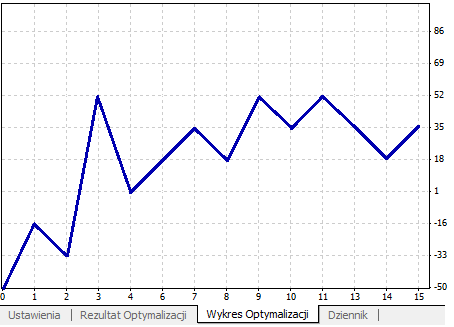
\includegraphics[width=12cm]{optymalizacja.png}
\caption{Wykres przedstawiający wyniki optymalizacji}
\label{wynikopt}
\end{center}
\end{figure} 
Powyższy przykład posiada trzy maksima, w teście trzecim, dziewiątym i jedenastym. Jeśli wykorzystując parametr z pierwszego maksimum zmniejszymy go lub zwiększymy o jeden krok to system będzie się zachowywał o wiele gorzej. Natomiast w przypadku drugiego i trzeciego maksimum, system jest mniej czuły na ewentualną zmianę o jeden krok. Wykorzystany powinien być zatem parametr z trzeciego maksimum, gdyż wtedy system jest najmniej wrażliwy na zmianę sytuacji rynkowej.

W przypadku optymalizacji dużej ilości parametrów zaleca się przeprowadzenie kilku optymalizacji na mniejszej ilości parametrów. Następnie po każdym procesie cząstkowej optymalizacji wybiera się najlepszy zestaw z uwzględnieniem jego wrażliwości na zmiany.
 
Po wyborze zbioru wartości parametrów, dla którego system uzyskuje najlepsze rezultaty, należy dodatkowo sprawdzić wygląd wykresu przebiegu kapitału. Często krok ten jest pomijany, przyjmując znaleziony zestaw parametrów za optymalny. Dwa różne przykłady linii kapitału przedstawiają wykresy poniżej.
\begin{figure}[h!]
\begin{center}
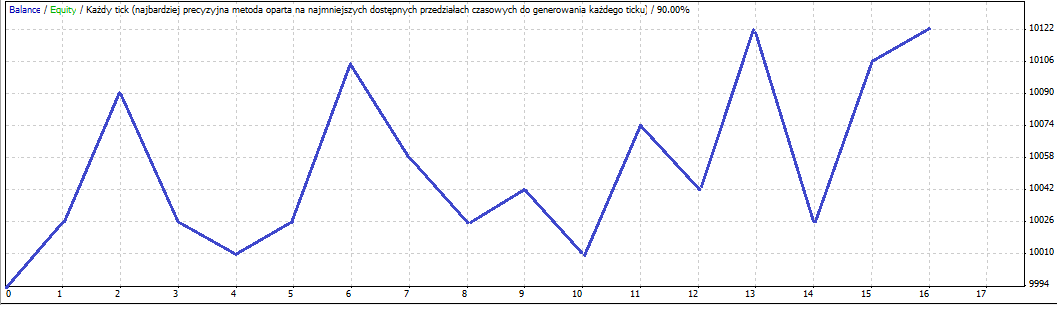
\includegraphics[width=12cm]{optymalizacja_zla.png}
\caption{Wykres przebiegu linii kapitału}
\label{liniakapzla}
\end{center}
\end{figure} 
\begin{figure}[h!]
\begin{center}
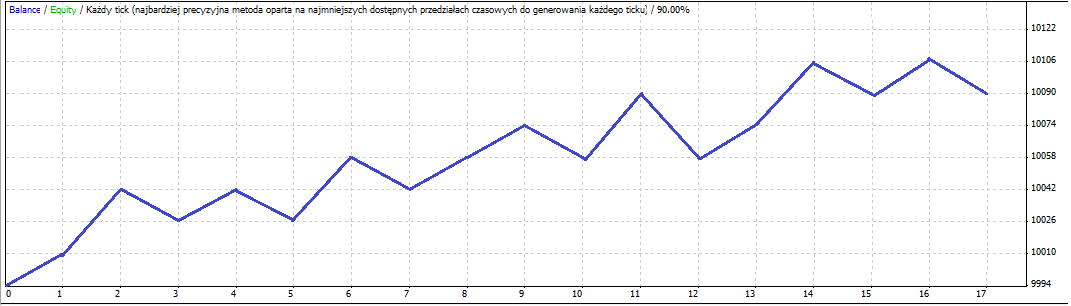
\includegraphics[width=12cm]{optymalizacja_dobra.png}
\caption{Wykres przebiegu linii kapitału}
\label{liniakapdobra}
\end{center}
\end{figure} 
W obu przypadkach został osiągnięty zysk. Jednak na wykresie \ref{liniakapzla} można zauważyć duże wahania kapitału. Gracz powinien natychmiast odrzucić ten zestaw parametrów i spróbować innego zestawu sugerowanego przez tester. Linia kapitału zachowuje się chaotycznie, skokowo wzrastając i opadając. Transakcje przynoszące duże zyski, są szybko niwelowane przez zlecenia stratne. Zachodzi więc podejrzenie, że system ten może dla różnych okresów czasu przynosić zupełnie różne rezultaty. Dodatkowo takie zachowanie się systemu może prowadzić do dużych strat w krótkim okresie czasu, a nawet wyzerowania konta inwestora. Drugi przypadek jest przykładem pożądanej linii kapitału. Długie serie zysków są przecinane krótkimi seriami strat, a zyski osiągane są równomiernie i stabilnie. Tego typu system teoretycznie będzie przynosił podobne zyski w różnych okresach czasu.

\section{Wyniki optymalizacji}
\paragraph{}



% itd.
% \appendix
% \include{dodatekA}
% \include{dodatekB}
% itd.

\bibliographystyle{plain}
\bibliography{bibliografia}


\end{document}
